% !TEX program = xelatex
% !TEX encoding = UTF-8 Unicode
%
%  LisPy Handbook — The Definitive Guide
%  Where Common Lisp and Python Become One
%
%  Author: Oscar Riveros — 2026
%  Build:  xelatex main.tex && xelatex main.tex
%

\documentclass{lispy-book}

\begin{document}

% ---------- front matter ----------
\frontmatter

\title{%
  {\Huge\bfseries\color{lispblue} LisPy Handbook}\\[6pt]
  {\Large\itshape The Definitive Guide}\\[4pt]
  {\large Where Common Lisp and Python Become One}\\[12pt]
  \rule{0.5\textwidth}{0.5pt}\\[8pt]
  {\small\itshape ``It is not Lisp. It is not Python. It is LisPy.''}
}
\author{Oscar Riveros}
\date{2026}

\maketitle
\thispagestyle{empty}

\clearpage

\vspace*{\fill}
\begin{center}
  \small
  Copyright~\textcopyright~2026 Oscar Riveros\\[6pt]
  All rights reserved.\\[12pt]
  \texttt{https://github.com/maxtuno/lispy}
\end{center}
\vspace*{\fill}

\clearpage

\tableofcontents
\clearpage

\listoffigures
\clearpage

\listoftables
\clearpage

% ---------- main matter ----------
\mainmatter

% ========================
% Part 0 — Preludio
% ========================
\part{Preludio}
\label{part:preludio}

\chapter{Manifiesto de LisPy}
\label{chap:manifesto}

LisPy nace de una convicción: no existe una razón técnica por la que un
programador deba elegir entre el poder expresivo de Lisp y el vasto
ecosistema de Python. La ingeniería de software moderna demanda ambos.

\section{La Visión}

LisPy integra dos runtimes en un mismo proceso: un intérprete de Common Lisp
escrito en C99 portable y el runtime embebido de CPython 3.14. El resultado
es un sistema donde las funciones de Lisp y Python conviven, se llaman
mutuamente y comparten memoria bajo un mismo techo de abstracción.

\section{¿Por qué Lisp?}

Lisp ofrece cualidades que ningún otro lenguaje iguala:

\begin{itemize}
\item \textbf{Expresividad máxima.} El código Lisp son datos (S-expressions),
  lo que permite metaprogramación sin precedentes mediante macros.
\item \textbf{Sistema de objetos (CLOS).} El Common Lisp Object System es el
  MOP (Meta-Object Protocol) más completo jamás diseñado, con métodos
  multimétodo, combinación de métodos y metamodelo reflejable.
\item \textbf{Sistema de condiciones.} El manejo de errores con
  \texttt{handler-case}, \texttt{handler-bind} y \texttt{restart-case}
  supera cualquier otro sistema de excepciones.
\item \textbf{Macros higiénicas.} La metaprogramación en tiempo de compilación
  permite crear DSLs (lenguajes de dominio específico) sin precedentes.
\end{itemize}

\section{¿Por qué Python?}

Python domina el panorama actual por razones igualmente sólidas:

\begin{itemize}
\item \textbf{Ecosistema.} NumPy, SciPy, scikit-learn, PyTorch, pandas,
  matplotlib -- ninguna plataforma científica iguala la madurez de Python.
\item \textbf{Comunidad.} Millones de desarrolladores, bibliotecas para todo.
\item \textbf{Rendimiento.} Aunque Python es lento como lenguaje, su ecosistema
  de extensiones nativas (C, Fortran, CUDA) ofrece velocidad nativa.
\end{itemize}

\section{¿Por qué Juntos?}

La combinación es cualitativamente superior a la suma de las partes. Lisp
orquesta y genera código; Python ejecuta cómputo intensivo. La comunicación
es bidireccional, con conversión automática de tipos y latencia
microscópica.

\section{Filosofía de Diseño}

LisPy se construye sobre principios claros:

\begin{itemize}
\item \textbf{Single-file C99 portable.} Todo el intérprete es un único
  archivo \texttt{lispy.c} de aproximadamente 66 000 líneas.
\item \textbf{CPython 3.14 embebido.} Sin DLLs externas ni dependencias
  frágiles: Python se linkea estáticamente.
\item \textbf{Puente bidireccional.} Lisp llama a Python y Python llama a
  Lisp con la misma naturalidad.
\item \textbf{Conversión automática.} Tipos Lisp y Python se convierten
  transparentemente siguiendo tablas bien definidas.
\end{itemize}

\section{Principio Rector}

\medskip
\begin{center}
\fbox{\parbox{0.8\textwidth}{\centering\itshape
Lisp como orquestador y generador,\\
Python como motor de cálculo.}}
\end{center}
\medskip

Este principio guía cada decisión de diseño: las partes del sistema que
requieren flexibilidad, metaprogramación y abstracción viven en Lisp. Las
partes que requieren cómputo numérico intensivo, acceso a bibliotecas
establecidas o procesamiento de datos delegan en Python.

\chapter{Cómo Leer Este Libro}
\label{chap:howtoread}

Este libro está organizado en capas: cada parte presupone el conocimiento de
las anteriores. Sin embargo, hemos marcado capítulos autocontenidos para
lectura no lineal.

\section{Notación y Convenciones}

Utilizamos las siguientes convenciones tipográficas:

\begin{itemize}
\item \texttt{\color{keywordblue} código Lisp} -- fragmentos de código
  Common Lisp en el intérprete LisPy.
\item \texttt{\color{keywordblue} código Python} -- fragmentos de código
  Python ejecutables desde LisPy.
\item \textbf{texto en negrita} -- términos nuevos o conceptos clave.
\item \textit{texto en cursiva} -- énfasis o referencias cruzadas.
\end{itemize}

\section{Símbolos de Dificultad}

Cada capítulo está marcado con estrellas que indican su nivel:

\begin{itemize}
\item $\bigstar$\!$\bigstar$\!$\bigstar$\!$\bigstar$ -- \textbf{Principiante.}
  No se requiere experiencia previa en Lisp ni Python.
\item $\bigstar$\!$\bigstar$\!$\bigstar$\!$\bigstar$ -- \textbf{Intermedio.}
  Presupone fundamentos de programación.
\item $\bigstar$\!$\bigstar$\!$\bigstar$\!$\bigstar$ -- \textbf{Avanzado.}
  Requiere comprensión de los conceptos presentados en partes anteriores.
\item $\bigstar$\!$\bigstar$\!$\bigstar$\!$\bigstar$ -- \textbf{Experto.}
  Material avanzado que presupone dominio de las secciones precedentes.
\end{itemize}

\section{Ejecución de Ejemplos}

Los ejemplos de código pueden ejecutarse de tres formas:

\begin{enumerate}
\item \textbf{Línea de comandos:} \texttt{lispy.exe ejemplo.lp}
\item \textbf{REPL interactivo:} \texttt{lispy.exe --repl}
\item \textbf{Evaluación directa:} \texttt{lispy.exe -e "(+ 1 2)"}
\end{enumerate}

\section{Dónde Encontrar el Código Fuente}

El código fuente de todas las librerías discutidas en el libro reside en el
directorio \texttt{lib/} de la distribución de LisPy:

\begin{itemize}
\item \texttt{lib/python-template.lp} -- generación de código Python
\item \texttt{lib/pythonic.lp} -- macro de transformación Lisp a Python
\item \texttt{lib/defpyfun.lp} -- funciones Python con captura Lisp
\item \texttt{lib/numpy-fast.lp} -- aceleración numérica vectorizada
\item \texttt{lib/defnp.lp} -- despacho automático vectorizado/escalar
\item \texttt{lib/sympy-bridge.lp} -- cálculo simbólico con SymPy
\item \texttt{lib/defmath.lp} -- matemáticas híbridas simbólico-numéricas
\item \texttt{lib/persist.lp} -- checkpoint/restore de sesión
\item \texttt{lib/continuations.lp} -- puente de corutinas
\item \texttt{lib/import-hooks.lp} -- transformación de AST
\item \texttt{lib/pandas-bridge.lp} -- DataFrames desde Lisp
\end{itemize}

\chapter{Hoja de Ruta del Aprendizaje}
\label{chap:roadmap}

Dependiendo de tu perfil y objetivos, recomendamos las siguientes rutas de
lectura. Cada ruta omite ciertos capítulos y enfatiza otros.

\section{Ruta A: Científico de Datos}

Esta ruta está diseñada para quienes desean usar LisPy como plataforma de
análisis de datos, computación científica y machine learning.

\begin{center}
\begin{tabular}{ll}
\toprule
\textbf{Parte} & \textbf{Capítulos} \\
\midrule
I -- Fundamentos & Todos \\
II -- El Núcleo Lisp & Capítulos 2.1, 2.2, 2.4 \\
III -- El Puente Python & Todos \\
IV -- Programación Híbrida & Todos \\
VI -- Matemáticas Aplicadas & Todos \\
VIII -- Estudios de Caso & Capítulos 8.3, 8.6 \\
\bottomrule
\end{tabular}
\end{center}

\section{Ruta B: Ingeniero de Software}

Para desarrolladores que buscan explotar la metaprogramación y la ingeniería
de sistemas.

\begin{center}
\begin{tabular}{ll}
\toprule
\textbf{Parte} & \textbf{Capítulos} \\
\midrule
I -- Fundamentos & Todos \\
II -- El Núcleo Lisp & Todos \\
V -- Meta-Programación & Todos \\
VII -- Ingeniería de Sistemas & Todos \\
VIII -- Estudios de Caso & Capítulos 8.2, 8.4, 8.7 \\
\bottomrule
\end{tabular}
\end{center}

\section{Ruta C: Matemático}

Para quienes se enfocan en matemáticas simbólicas, numéricas y sus
aplicaciones.

\begin{center}
\begin{tabular}{ll}
\toprule
\textbf{Parte} & \textbf{Capítulos} \\
\midrule
I -- Fundamentos & Todos \\
III -- El Puente Python & Todos \\
VI -- Matemáticas Aplicadas & Todos \\
VIII -- Estudios de Caso & Capítulo 8.1 \\
\bottomrule
\end{tabular}
\end{center}

\section{Ruta D: Hacker de Lenguajes}

Para entusiastas de la metaprogramación y el diseño de lenguajes.

\begin{center}
\begin{tabular}{ll}
\toprule
\textbf{Parte} & \textbf{Capítulos} \\
\midrule
I -- Fundamentos & Todos \\
II -- El Núcleo Lisp & Todos \\
V -- Meta-Programación & Todos \\
VII -- Ingeniería de Sistemas & Capítulos 7.1, 7.4 \\
\bottomrule
\end{tabular}
\end{center}

\section{Ruta E: Principiante Absoluto}

\begin{enumerate}
\item Completar la Parte I (Fundamentos) completamente.
\item Elegir una ruta especializada según intereses.
\item Volver a capítulos omitidos cuando sea necesario.
\end{enumerate}

Cada ruta está diseñada para ser completa en sí misma, proporcionando tanto
profundidad como amplitud en el área de enfoque.

\chapter{Mapa de Dependencias entre Capítulos}
\label{chap:deps}

Este capítulo describe el grafo de prerrequisitos entre capítulos,
permitiendo al lector planificar una lectura no lineal cuando sea necesario.

\section{Base Universal}

La Parte I (Fundamentos) es el único punto de entrada verdadero. No tiene
dependencias previas y es requisito para todas las demás partes.

\section{Dependencias por Parte}

\begin{itemize}
\item \textbf{Parte II} (El Núcleo Lisp) depende de la Parte I: sintaxis,
  tipos, control de flujo.
\item \textbf{Parte III} (El Puente Python) depende de las Partes I y II:
  funciones, símbolos, macros.
\item \textbf{Parte IV} (Programación Híbrida) depende de las Partes I, II y
  III: puente Python, CLOS, macros.
\item \textbf{Parte V} (Meta-Programación) depende de las Partes I--IV.
\item \textbf{Parte VI} (Matemáticas Aplicadas) depende de las Partes I, III
  y IV: \texttt{numpy-fast}, \texttt{sympy-bridge}, \texttt{defmath}.
\item \textbf{Parte VII} (Ingeniería de Sistemas) depende de las Partes I y
  II: compilación, CLI, sistema.
\item \textbf{Parte VIII} (Estudios de Caso) depende de las Partes I--VI
  según el caso de estudio específico.
\end{itemize}

\section{Matriz de Prerrequisitos}

\begin{center}
\small
\begin{tabular}{lccccccccc}
\toprule
\textbf{Capítulo} & \textbf{I} & \textbf{II} & \textbf{III} & \textbf{IV} & \textbf{V} & \textbf{VI} & \textbf{VII} \\
\midrule
I (1.1--1.8) & -- & -- & -- & -- & -- & -- & -- \\
II (2.1--2.9) & $\bullet$ & -- & -- & -- & -- & -- & -- \\
III (3.1--3.9) & $\bullet$ & $\bullet$ & -- & -- & -- & -- & -- \\
IV (4.1--4.11) & $\bullet$ & $\bullet$ & $\bullet$ & -- & -- & -- & -- \\
V (5.1--5.8) & $\bullet$ & $\bullet$ & $\bullet$ & $\bullet$ & -- & -- & -- \\
VI (6.1--6.8) & $\bullet$ & -- & $\bullet$ & $\bullet$ & -- & -- & -- \\
VII (7.1--7.7) & $\bullet$ & $\bullet$ & -- & -- & -- & -- & -- \\
VIII (8.1--8.7) & $\bullet$ & $\bullet$ & $\bullet$ & $\bullet$ & $\circ$ & $\circ$ & $\circ$ \\
\bottomrule
\end{tabular}
\end{center}

Leyenda: $\bullet$ = requisito directo, $\circ$ = requisito parcial.

\section{Capítulos Autocontenidos}

Los siguientes capítulos pueden leerse de forma independiente, marcados con
$(*)$ para lectura no lineal:

\begin{itemize}
\item Capítulo 2.7 -- LOOP avanzado $(*)$
\item Capítulo 3.9 -- FFI directa $(*)$
\item Capítulo 4.8 -- Persistencia $(*)$
\item Capítulo 7.3 -- Gestión de paquetes pip $(*)$
\item Capítulo 7.5 -- Pruebas $(*)$
\end{itemize}

\section{Recomendación de Orden}

Para cada ruta de aprendizaje (ver Capítulo~\ref{chap:roadmap}, se recomienda
seguir el orden numérico dentro de las partes seleccionadas. Los capítulos
autocontenidos pueden intercalarse según el interés del lector.


% ========================
% Part I — Fundamentos
% ========================
\part{Fundamentos}
\label{part:fundamentos}

\chapter{Instalación y Primeros Pasos}
\label{chap:installation}

{\huge$\bigstar$} Principiante

\section{Requisitos del Sistema}

LisPy está diseñado para Windows x64. Los requisitos mínimos son:

\begin{itemize}
\item Sistema operativo: Windows 10 o superior (x64)
\item Opcional: CPython 3.14 instalado (para soporte completo del puente Python)
\item Espacio en disco: ~50 MB para la instalación base
\end{itemize}

\section{Descarga e Instalación}

Descarga el binario \texttt{lispy.exe} desde el repositorio oficial y
colócalo en un directorio de tu elección. Opcionalmente, añade dicho
directorio a la variable de entorno \texttt{PATH} para acceso global.

\section{Verificación}

Abre una terminal y ejecuta:

\begin{lispcode}
lispy.exe --version
\end{lispcode}

Deberías ver información sobre la versión y configuración del intérprete.

\section{Entornos Virtuales Python}

Si deseas aislar las dependencias Python de tu proyecto:

\begin{lstlisting}[style=python,title=Terminal]
python -m venv mi_entorno
lispy.exe --venv mi_entorno
\end{lstlisting}

\section{Primer Comando}

Inicia el REPL:

\begin{lstlisting}[style=python,title=Terminal]
lispy.exe --repl
\end{lstlisting}

En el prompt \texttt{LisPy>}, escribe:

\begin{lispcode}
(+ 1 2)
\end{lispcode}

LisPy responderá con \texttt{3}.

\section{El REPL Interactivo}

El REPL de LisPy ofrece los siguientes comandos:

\begin{itemize}
\item \texttt{:help} -- Muestra la ayuda del REPL
\item \texttt{:quit} -- Sale del REPL
\item \texttt{:pip} -- Gestión de paquetes Python
\item \texttt{:trace} -- Activa/desactiva traza de ejecución
\end{itemize}

\section{Ejemplos}

\begin{examplebox}
\begin{lispcode}
;; hello.lp - Primer programa
(format t "Hello, LisPy!~%")
\end{lispcode}
Salida: \texttt{Hello, LisPy!}
\end{examplebox}

\begin{examplebox}
\begin{lispcode}
;; Uso de --venv con un entorno virtual preexistente
;; Terminal:
;;   lispy.exe --venv mi_entorno script.lp

;; Instalación de numpy desde el REPL
;; LisPy> :pip install numpy
\end{lispcode}
\end{examplebox}


\chapter{Átomos y Tipos de Datos Primitivos}
\label{chap:atoms}

{\huge$\bigstar$} Principiante

Todo valor en LisPy es, en última instancia, un átomo o una celda cons. Este
capítulo cubre los tipos atómicos fundamentales.

\section{Números Enteros}

Los enteros en LisPy tienen precisión arbitraria (bigints):

\begin{lispcode}
42
-7
123456789012345678901234567890
\end{lispcode}

No hay desbordamiento: un entero puede tener tantos dígitos como la memoria
lo permita.

\section{Números Racionales}

Los racionales se escriben como fracción:

\begin{lispcode}
1/3
22/7
\end{lispcode}

Las operaciones aritméticas entre racionales producen resultados exactos:

\begin{lispcode}
(+ 1/3 1/7 1/11)  ;; → 137/231
\end{lispcode}

\section{Números Flotantes}

Los flotantes siguen el estándar IEEE 754 de doble precisión:

\begin{lispcode}
3.14159
1.0e10
-0.5
\end{lispcode}

\section{Números Complejos}

Los números complejos se construyen con la notación \texttt{\#C}:

\begin{lispcode}
#C(3 4)       ;; 3 + 4i
#C(1.0 -2.5)  ;; 1.0 - 2.5i
\end{lispcode}

\section{Caracteres}

Los caracteres se escriben con la sintaxis \texttt{\#\textbackslash}:

\begin{lispcode}
#\A          ;; la letra A mayúscula
#\Space      ;; el carácter de espacio
#\Newline    ;; el carácter de nueva línea
#\λ          ;; lambda griega (Unicode)
\end{lispcode}

\section{Strings}

Las cadenas se delimitan con comillas dobles:

\begin{lispcode}
"Hello"
"Línea 1~%Línea 2"  ;; ~% inserta un salto de línea
\end{lispcode}

\section{Símbolos}

Los símbolos son identificadores con nombre. Se escriben con comilla simple
para evitar su evaluación:

\begin{lispcode}
'foo                      ;; el símbolo FOO
'|nombre con espacios|    ;; símbolo con espacios internos
:keyword                  ;; keyword (símbolo en el paquete KEYWORD)
\end{lispcode}

\section{Booleanos}

\begin{lispcode}
t    ;; verdadero
nil  ;; falso (también la lista vacía)
\end{lispcode}

En Common Lisp, \texttt{nil} es el único valor falso; cualquier otro valor es
verdadero en contexto booleano.

\section{Conversión entre Tipos}

\begin{lispcode}
(float 42)           ;; → 42.0
(coerce 3/2 'float)  ;; → 1.5
(numerator 3/2)      ;; → 3
(denominator 3/2)    ;; → 2
\end{lispcode}

\section{Ejemplos}

\begin{examplebox}[title=Precisión arbitraria]
\begin{lispcode}
;; Fibonacci(100)
(defun fib (n)
  (if (< n 2) n
    (+ (fib (- n 1)) (fib (- n 2)))))
;; Nota: usar versión iterativa para valores grandes
\end{lispcode}
\end{examplebox}

\begin{examplebox}[title=Aritmética exacta con racionales]
\begin{lispcode}
(+ 1/3 1/7 1/11)  ;; fracción exacta: 137/231
(* 1/3 3)         ;; → 1
\end{lispcode}
\end{examplebox}

\begin{examplebox}[title=Números complejos]
\begin{lispcode}
(* #C(3 4) #C(1 -2))  ;; → #C(11 -2)
(abs #C(3 4))         ;; → 5.0 (magnitud)
(phase #C(1 1))       ;; → 0.785398... (fase en radianes)
\end{lispcode}
\end{examplebox}


\chapter{Listas: La Estructura de Datos Universal}
\label{chap:lists}

{\huge$\bigstar$} Principiante

En Lisp, las listas son la estructura de datos fundamental. Toda la sintaxis
del lenguaje se reduce a listas (S-expressions), lo que hace que el código
sea datos y los datos sean código.

\section{Celdas Cons}

La celda cons es el bloque constructor de las listas:

\begin{lispcode}
(cons 1 2)  ;; → (1 . 2)  — dotted pair
\end{lispcode}

Una lista propia es una cadena de celdas cons donde la última apunta a nil:

\begin{lispcode}
(cons 1 (cons 2 (cons 3 nil)))  ;; → (1 2 3)
'(1 2 3 4 5)                     ;; notación literal
(list 1 2 3)                     ;; constructor
\end{lispcode}

\section{Operaciones de Acceso}

\begin{lispcode}
(car '(1 2 3))    ;; → 1  (first)
(cdr '(1 2 3))    ;; → (2 3)  (rest)
(cadr '(1 2 3))   ;; → 2  (second)
(caddr '(1 2 3))  ;; → 3  (third)
(nth 2 '(a b c))  ;; → C
\end{lispcode}

\section{Operaciones de Construcción}

\begin{lispcode}
(push 'x lista)          ;; añade x al inicio
(pop lista)              ;; extrae y retorna el primer elemento
(pushnew 'x lista)       ;; añade si no existe
(append '(1 2) '(3 4))   ;; → (1 2 3 4)
(list* 1 2 '(3 4))       ;; → (1 2 3 4)
(make-list 5 :initial-element 0)  ;; → (0 0 0 0 0)
\end{lispcode}

\section{Búsqueda en Listas}

\begin{lispcode}
(member 3 '(1 2 3 4) :test #'=)       ;; → (3 4)
(find 'c '(a b c d) :test #'eq)       ;; → C
(position 3 '(1 2 3 4 5))              ;; → 2
\end{lispcode}

\section{Listas de Asociación (Alists)}

\begin{lispcode}
(defvar *productos*
  '((:manzana . 0.50)
    (:pan . 2.00)
    (:leche . 1.20)))

(assoc :pan *productos*)   ;; → (:PAN . 2.00)
(rassoc 1.20 *productos*)  ;; → (:LECHE . 1.20)
\end{lispcode}

\section{Operaciones de Conjuntos}

\begin{lispcode}
(adjoin 3 '(1 2 3 4))                ;; → (1 2 3 4) (sin duplicados)
(union '(1 2 3) '(2 3 4))            ;; → (1 2 3 4)
(intersection '(1 2 3) '(2 3 4))     ;; → (2 3)
(set-difference '(1 2 3) '(2 3 4))   ;; → (1)
\end{lispcode}

\section{Ejemplos}

\begin{examplebox}[title=Construcción incremental con push/pop]
\begin{lispcode}
(defvar *pila* nil)
(push 10 *pila*)     ;; → (10)
(push 20 *pila*)     ;; → (20 10)
(pop *pila*)         ;; → 20, *pila* → (10)
(pop *pila*)         ;; → 10, *pila* → nil
\end{lispcode}
\end{examplebox}

\begin{examplebox}[title=Base de datos de productos con alists]
\begin{lispcode}
(defvar *db*
  '((:producto-1 :nombre "Laptop" :precio 1200)
    (:producto-2 :nombre "Mouse"  :precio 25)))

(defun buscar-precio (id)
  (let ((entry (assoc id *db*)))
    (when entry
      (getf (cdr entry) :precio))))

(buscar-precio :producto-1)  ;; → 1200
\end{lispcode}
\end{examplebox}

\begin{examplebox}[title=Aplanamiento recursivo]
\begin{lispcode}
(defun flatten (lst)
  (if (null lst)
      nil
      (if (listp (car lst))
          (append (flatten (car lst))
                  (flatten (cdr lst)))
          (cons (car lst) (flatten (cdr lst))))))

(flatten '((1 2) (3 (4 5)) 6))  ;; → (1 2 3 4 5 6)
\end{lispcode}
\end{examplebox}

\begin{examplebox}[title=Zip de dos listas]
\begin{lispcode}
(defun zip (a b)
  (if (or (null a) (null b))
      nil
      (cons (cons (car a) (car b))
            (zip (cdr a) (cdr b)))))

(zip '(1 2 3) '(a b c))  ;; → ((1 . A) (2 . B) (3 . C))
\end{lispcode}
\end{examplebox}


\chapter{Vectores y Secuencias}
\label{chap:vectors}
{\huge$\bigstar$} Principiante

\section{Vectores}
\begin{lispcode}
#(1 2 3)
(vector 1 2 3)
(make-array 5 :initial-element 0)
\end{lispcode}

\section{Acceso Indexado}
\begin{lispcode}
(aref #(10 20 30) 1)
(let ((v (vector 1 2 3))) (setf (aref v 1) 99) v)
\end{lispcode}

\section{Vectores Ajustables}
\begin{lispcode}
(defvar *buf* (make-array 3 :fill-pointer 0 :initial-element nil))
(vector-push 'a *buf*)
(vector-pop *buf*)
\end{lispcode}

\section{Operaciones sobre Secuencias}
\begin{lispcode}
(length #(1 2 3))
(elt #(10 20 30) 1)
(subseq #(1 2 3 4 5) 1 3)
(fill #(1 2 3) 0)
(reverse #(1 2 3))
\end{lispcode}

\section{Reduce}
\begin{lispcode}
(reduce #'+ #(1 2 3 4 5))
(reduce #'max #(3 1 4 1 5))
\end{lispcode}

\section{Búsqueda y Filtrado}
\begin{lispcode}
(count 2 #(1 2 2 3 2))
(remove-if #'evenp #(1 2 3 4 5))
(find-if #'oddp #(2 4 5 6))
\end{lispcode}

\section{Ordenamiento}
\begin{lispcode}
(sort #(3 1 4 1 5) #'<)
(sort #((:a 3) (:b 1) (:c 2)) #'< :key #'second)
\end{lispcode}

\begin{examplebox}[title=Producto escalar con reduce]
\begin{lispcode}
(defun dot-product (a b)
  (reduce #'+ (map 'vector #'* a b)))
(dot-product #(1 2 3) #(4 5 6))
\end{lispcode}
\end{examplebox}


\chapter{Hash Tables y Diccionarios}
\label{chap:hashtables}
{\huge$\bigstar$} Principiante

\section{Creación y Operaciones Básicas}
\begin{lispcode}
(defvar *ht* (make-hash-table :test 'equal))
(setf (gethash "clave" *ht*) "valor")
(gethash "clave" *ht*)
(remhash "clave" *ht*)
(clrhash *ht*)
\end{lispcode}

\section{Tests de Comparación}
\paragraph{:test} determine cómo se comparan las claves: \texttt{eq},
\texttt{eql}, \texttt{equal}, \texttt{equalp}.

\section{Iteración}
\begin{lispcode}
(maphash (lambda (k v) (format t "~A → ~A~%" k v)) *ht*)
(hash-table-count *ht*)
(hash-table-p *ht*)
\end{lispcode}

\begin{examplebox}[title=Contador de palabras]
\begin{lispcode}
(defun word-count (words)
  (let ((ht (make-hash-table :test 'equal)))
    (dolist (w words ht)
      (incf (gethash w ht 0)))))
(word-count '("the" "quick" "brown" "fox" "the"))
\end{lispcode}
\end{examplebox}

\begin{examplebox}[title=Memoización de Fibonacci]
\begin{lispcode}
(defvar *fib-cache* (make-hash-table :test 'eql))
(defun fib-fast (n)
  (or (gethash n *fib-cache*)
      (setf (gethash n *fib-cache*)
            (if (< n 2) n (+ (fib-fast (- n 1)) (fib-fast (- n 2)))))))
(fib-fast 100)
\end{lispcode}
\end{examplebox}

\begin{examplebox}[title=Two-sum con hash table]
\begin{lispcode}
(defun two-sum (nums target)
  (let ((seen (make-hash-table :test 'eql)))
    (dotimes (i (length nums))
      (let ((complement (- target (aref nums i))))
        (multiple-value-bind (found idx) (gethash complement seen)
          (when found (return-from two-sum (list idx i)))))
      (setf (gethash (aref nums i) seen) i))
    nil))
(two-sum #(2 7 11 15) 9)
\end{lispcode}
\end{examplebox}


\chapter{Control de Flujo Básico}
\label{chap:control}
{\huge$\bigstar$} Principiante

\section{Condicionales}
\begin{lispcode}
(if (> x 0) "positivo" "no positivo")
(when (> x 0) (print "es positivo"))
(unless (= x 0) (print "x no es cero"))
\end{lispcode}

\section{Cond}
\begin{lispcode}
(cond ((< x 0) "negativo") ((= x 0) "cero") (t "positivo"))
\end{lispcode}

\section{Case y Typecase}
\begin{lispcode}
(case char (#\+ :sumar) (#\- :restar) (otherwise :desconocido))
\end{lispcode}

\section{Asignación}
\begin{lispcode}
(setq x 10)
(setf (aref v 0) 5)
(incf x) (decf x)
(rotatef a b)
\end{lispcode}

\section{Asignación Paralela}
\begin{lispcode}
(psetf a b b a)
(psetq x 1 y 2)
\end{lispcode}

\begin{examplebox}[title=Calculadora de tarifas con cond]
\begin{lispcode}
(defun tarifa (edad)
  (cond ((< edad 5) 0) ((< edad 18) 5.0) ((< edad 65) 10.0) (t 7.5)))
(tarifa 30) (tarifa 70)
\end{lispcode}
\end{examplebox}

\begin{examplebox}[title=Intercambio con rotatef]
\begin{lispcode}
(let ((a 10) (b 20)) (rotatef a b) (list a b))
\end{lispcode}
\end{examplebox}


\chapter{Iteración y Recursión}
\label{chap:iteration}
{\huge$\bigstar$} Principiante

\section{Iteración Simple}
\begin{lispcode}
(dotimes (i 5) (print i))
(dolist (x '(a b c)) (print x))
\end{lispcode}

\section{LOOP}
\begin{lispcode}
(loop for i from 1 to 5 collect (* i i))
(loop for x in '(3 1 4 1 5) sum x)
(loop for x in '(3 1 4 1 5) maximize x)
\end{lispcode}

\section{DO y DO*}
\begin{lispcode}
(do ((i 0 (1+ i)) (sum 0 (+ sum i))) ((> i 10) sum) (print i))
\end{lispcode}

\section{Recursión}
\begin{lispcode}
(defun factorial (n) (if (<= n 1) 1 (* n (factorial (- n 1)))))
(defun factorial-tail (n)
  (labels ((iter (acc m) (if (<= m 1) acc (iter (* acc m) (- m 1)))))
    (iter 1 n)))
\end{lispcode}

\section{Salida No Local}
\begin{lispcode}
(block busqueda
  (dotimes (i 10) (dotimes (j 10) (if (= i j 5) (return-from busqueda (list i j))))))
(catch 'found
  (dolist (x '(1 2 3 4 5)) (if (= x 3) (throw 'found :encontrado) (print x))))
\end{lispcode}

\begin{examplebox}[title=LOOP para Project Euler \#1]
\begin{lispcode}
(defun euler-1 ()
  (loop for i from 1 below 1000
        when (or (= (mod i 3) 0) (= (mod i 5) 0)) sum i))
\end{lispcode}
\end{examplebox}

\begin{examplebox}[title=MCD con DO*]
\begin{lispcode}
(defun mcd (a b) (do* ((x a y) (y b (mod x y))) ((= y 0) x)))
(mcd 48 18)
\end{lispcode}
\end{examplebox}


\chapter{Entrada/Salida Fundamental}
\label{chap:io}
{\huge$\bigstar$} Principiante

\section{La Función Format}
\begin{lispcode}
(format t "~A~%" "Hola")
(format nil "~A + ~A = ~A" 1 2 3)
(format nil "~D" 42)
(format nil "~B" 42)
(format nil "~X" 255)
(format nil "~5,2F" 3.14159)
(format nil "~@R" 42)
\end{lispcode}

\section{Print y Variantes}
\begin{lispcode}
(print "Hola") (princ "Hola") (prin1 "Hola") (terpri)
\end{lispcode}

\section{Lectura}
\begin{lispcode}
(let ((x (read))) (format t "Leí: ~A" x))
(read-line) (read-char) (read-from-string "(+ 1 2)")
\end{lispcode}

\section{Archivos}
\begin{lispcode}
(with-open-file (out "salida.txt" :direction :output :if-exists :supersede)
  (format out "Hola, archivo~%"))
(with-open-file (in "entrada.txt" :direction :input)
  (let ((c (read-line in nil nil))) c))
\end{lispcode}

\section{Redirección de Streams}
\begin{lispcode}
(with-output-to-string (out) (format out "Esto va al string"))
(with-input-from-string (in "(1 2 3)") (read in))
\end{lispcode}

\begin{examplebox}[title=Formato tabular]
\begin{lispcode}
(defun tabla-cuadrados (&optional (n 10))
  (format t "~&~@A~20@A~30@A~%" "N" "N^2" "N^3")
  (dotimes (i n)
    (let ((x (1+ i)))
      (format t "~&~D~20@D~30@D~%" x (* x x) (* x x x)))))
\end{lispcode}
\end{examplebox}



% ========================
% Part II — El Núcleo Lisp
% ========================
\part{El Núcleo Lisp}
\label{part:nuclisp}

\chapter{Funciones y Ámbitos}
\label{chap:functions}
{\huge$\bigstar$}{\huge$\bigstar$} Intermedio

\section{Definición de Funciones}
\begin{lispcode}
(defun cuadrado (x) (* x x))
\end{lispcode}

\section{Parámetros}
\begin{lispcode}
(defun saludar (nombre &optional (saludo "Hola"))
  (format t "~A, ~A~%" saludo nombre))
(defun suma (&rest numeros) (reduce #'+ numeros))
(defun crear-punto (&key (x 0) (y 0)) (cons x y))
\end{lispcode}

\section{Funciones Anónimas}
\begin{lispcode}
(lambda (x) (* x x))
#'(lambda (x) (* x x))
\end{lispcode}

\section{Funciones Locales}
\begin{lispcode}
(flet ((doble (x) (* x 2)) (triple (x) (* x 3))) (+ (doble 5) (triple 5)))
(labels ((par? (n) (if (= n 0) t (impar? (1- n))))
         (impar? (n) (if (= n 0) nil (par? (1- n)))))
  (par? 4))
\end{lispcode}

\section{Closures}
\begin{lispcode}
(defun make-contador (&optional (inicial 0))
  (let ((cuenta inicial)) (lambda () (incf cuenta))))
(defvar *c* (make-contador 10))
(funcall *c*)
\end{lispcode}

\section{Múltiples Valores}
\begin{lispcode}
(values 10 20 30)
(multiple-value-bind (a b c) (values 1 2 3) (list a b c))
\end{lispcode}

\begin{examplebox}[title=Contador con estado encapsulado]
\begin{lispcode}
(defun make-acumulador ()
  (let ((total 0)) (lambda (n) (incf total n))))
\end{lispcode}
\end{examplebox}

\begin{examplebox}[title=Divmod con múltiples valores]
\begin{lispcode}
(defun divmod (a b) (values (floor a b) (mod a b)))
(multiple-value-bind (c r) (divmod 17 5) (list c r))
\end{lispcode}
\end{examplebox}


\chapter{Símbolos, Paquetes y Namespaces}
\label{chap:packages}
{\huge$\bigstar$}{\huge$\bigstar$} Intermedio

\section{Símbolos}
\begin{lispcode}
(intern "FOO")
(make-symbol "FOO")
(gensym "TEMP")
(symbol-name 'foo)
(symbol-package 'foo)
(boundp 'x)
(fboundp 'car)
\end{lispcode}

\section{Property Lists}
\begin{lispcode}
(setf (get 'persona :nombre) "Juan")
(symbol-plist 'persona)
(remprop 'persona :edad)
\end{lispcode}

\section{Paquetes}
\begin{lispcode}
(defpackage :mi-paquete (:use :common-lisp) (:export :funcion-exportada))
(in-package :mi-paquete)
(defun funcion-exportada () "visible fuera")
\end{lispcode}

\section{El Paquete PYTHON}
\begin{lispcode}
(find-package :py)
(find-package :python)
\end{lispcode}

\begin{examplebox}[title=Gensym para higiene en macros]
\begin{lispcode}
(defmacro con-temp ((var valor) &body body)
  (let ((g (gensym)))
    `(let ((,g ,valor)) (let ((,var ,g)) ,@body))))
\end{lispcode}
\end{examplebox}


\chapter{Macros: Metaprogramación en Tiempo de Compilación}
\label{chap:macros}
{\huge$\bigstar$}{\huge$\bigstar$} Intermedio

\section{Sintaxis Básica}
\begin{lispcode}
(defmacro macro-name (&rest args) cuerpo-de-expansión)
\end{lispcode}

\section{Quasiquoting}
\begin{lispcode}
(defmacro suma-cuadrados (a b) `(+ (* ,a ,a) (* ,b ,b)))
(macroexpand-1 '(suma-cuadrados 3 4))
\end{lispcode}

\section{Higiene con Gensym}
\begin{lispcode}
(defmacro con-temp ((var valor) &body body)
  (let ((g (gensym)))
    `(let ((,g ,valor)) (let ((,var ,g)) ,@body))))
\end{lispcode}

\section{Macro Anafórica}
\begin{lispcode}
(defmacro aif (test then &optional else)
  `(let ((it ,test)) (if it ,then ,else)))
\end{lispcode}

\section{Compilador Macros}
\begin{lispcode}
(defun cuadrado (x) (* x x))
(define-compiler-macro cuadrado (x)
  (if (numberp x) `(* ,x ,x) `(cuadrado ,x)))
\end{lispcode}

\begin{examplebox}[title=Macro while personalizada]
\begin{lispcode}
(defmacro while (test &body body)
  `(do () ((not ,test)) ,@body))
(let ((x 5) (result nil))
  (while (> x 0) (push x result) (decf x))
  (nreverse result))
\end{lispcode}
\end{examplebox}

\begin{examplebox}[title=Destructuring con with-coords]
\begin{lispcode}
(defmacro with-coords ((x y) point &body body)
  `(let ((,x (car ,point)) (,y (cadr ,point))) ,@body))
(with-coords (a b) '(10 20) (+ a b))
\end{lispcode}
\end{examplebox}


\chapter{CLOS: Common Lisp Object System (Fundamentos)}
\label{chap:clos-basics}
{\huge$\bigstar$}{\huge$\bigstar$} Intermedio

\section{Definición de Clases}
\begin{lispcode}
(defclass punto ()
  ((x :initarg :x :initform 0 :accessor punto-x)
   (y :initarg :y :initform 0 :accessor punto-y)))
(defclass punto-3d (punto) ((z :initarg :z :initform 0 :accessor punto-z)))
\end{lispcode}

\section{Creación de Instancias}
\begin{lispcode}
(defvar *p* (make-instance 'punto :x 3 :y 4))
(punto-x *p*)
(setf (punto-x *p*) 5)
(slot-value *p* 'y)
\end{lispcode}

\section{Acceso Conciso}
\begin{lispcode}
(defmethod mostrar ((p punto))
  (with-slots (x y) p (format t "Punto(~D, ~D)~%" x y)))
\end{lispcode}

\section{Funciones Genéricas}
\begin{lispcode}
(defgeneric area (figura))
(defmethod area ((p punto)) 0)
(defmethod area ((c circulo)) (* pi (expt (circulo-radio c) 2)))
\end{lispcode}

\section{Especializadores EQL}
\begin{lispcode}
(defgeneric tasa-impuesto (pais))
(defmethod tasa-impuesto ((pais (eql :us))) 0.15)
(defmethod tasa-impuesto ((pais (eql :uk))) 0.20)
(defmethod tasa-impuesto (pais) 0.25)
\end{lispcode}

\begin{examplebox}[title=Jerarquía de figuras geométricas]
\begin{lispcode}
(defclass shape () ((color :initarg :color :initform :black)))
(defclass circle (shape) ((radius :initarg :radius :initform 1)))
(defclass rectangle (shape) ((width :initarg :width :initform 1) (height :initarg :height :initform 1)))
\end{lispcode}
\end{examplebox}

\begin{examplebox}[title=Change-class para migración]
\begin{lispcode}
(defclass point-2d () ((x :initarg :x) (y :initarg :y)))
(defclass point-3d (point-2d) ((z :initarg :z :initform 0)))
(let ((p (make-instance 'point-2d :x 1 :y 2)))
  (change-class p 'point-3d)
  (list (px p) (py p) (pz p)))
\end{lispcode}
\end{examplebox}


\chapter{CLOS Avanzado: Combinación de Métodos}
\label{chap:clos-advanced}
{\huge$\bigstar$}{\huge$\bigstar$} Intermedio

\section{Métodos Auxiliares}
\begin{lispcode}
(defgeneric procesar (x))
(defmethod procesar :before ((x numero)) (format t "Antes~%"))
(defmethod procesar :after ((x numero)) (format t "Después~%"))
(defmethod procesar ((x numero)) (* x x))
\end{lispcode}

\section{Orden de Ejecución}
\begin{enumerate}
\item \texttt{:around} (más específico primero)
\item \texttt{:before} (más específico primero)
\item Método primario
\item \texttt{:after} (más específico último)
\end{enumerate}

\section{Métodos Around}
\begin{lispcode}
(defmethod procesar :around ((x integer))
  (format t "Around~%")
  (let ((r (call-next-method))) (* r 2)))
\end{lispcode}

\section{Herencia Múltiple}
\begin{lispcode}
(defclass a () ((val :initform "A")))
(defclass b () ((val :initform "B")))
(defclass c (a b) ())
\end{lispcode}

\begin{examplebox}[title=Middleware pipeline]
\begin{lispcode}
(defgeneric handle-request (req))
(defmethod handle-request :around (req)
  (format t "Log: ~A~%" req) (let ((r (call-next-method))) r))
(defmethod handle-request :before (req) (format t "Validando~%"))
(defmethod handle-request ((req string)) :ok)
\end{lispcode}
\end{examplebox}


\chapter{Sistema de Condiciones y Re-inicios}
\label{chap:conditions}
{\huge$\bigstar$}{\huge$\bigstar$} Intermedio

\section{Condicionales Básicos}
\begin{lispcode}
(error "Algo salió mal")
(warn "Esto es una advertencia")
(cerror "Continuar" "Error no crítico")
\end{lispcode}

\section{Handler-Case}
\begin{lispcode}
(handler-case (/ 1 0)
  (division-by-zero (c) (format t "Capturado: ~A~%" c) :infinito))
\end{lispcode}

\section{Handler-Bind}
\begin{lispcode}
(handler-bind ((warning #'(lambda (c) (format t "Advertencia~%") (muffle-warning c))))
  (warn "Alerta"))
\end{lispcode}

\section{Limpieza Garantizada}
\begin{lispcode}
(unwind-protect (progn (abrir-recurso) (procesar)) (cerrar-recurso))
\end{lispcode}

\section{Condiciones Personalizadas}
\begin{lispcode}
(define-condition malformed-input (error) ((input :initarg :input)))
(error 'malformed-input :input "bad!")
\end{lispcode}

\begin{examplebox}[title=División segura]
\begin{lispcode}
(defun safe-div (a b)
  (handler-case (values (/ a b) nil)
    (division-by-zero (c) (values 0 c))))
\end{lispcode}
\end{examplebox}


\chapter{Iteración Avanzada y LOOP}
\label{chap:loop-advanced}
{\huge$\bigstar$}{\huge$\bigstar$} Intermedio

\section{Recorrido de Secuencias}
\begin{lispcode}
(loop for x in '(1 2 3 4 5) collect x)
(loop for x across \#(1 2 3) collect x)
\end{lispcode}

\section{Rangos Numéricos}
\begin{lispcode}
(loop for i from 1 to 5 collect i)
(loop for i from 1 below 5 collect i)
(loop for i from 1 to 10 by 2 collect i)
\end{lispcode}

\section{Acumulación}
\begin{lispcode}
(loop for x in '(3 1 4 1 5) sum x)
(loop for x in '(3 1 4 1 5) maximize x)
\end{lispcode}

\section{Condicionales en LOOP}
\begin{lispcode}
(loop for x in '(1 2 3 4 5 6) when (evenp x) collect (* x x))
\end{lispcode}

\begin{examplebox}[title=Fibonacci con = y then]
\begin{lispcode}
(loop for a = 1 then b for b = 1 then (+ a b) repeat 10 collect a)
\end{lispcode}
\end{examplebox}

\begin{examplebox}[title=LOOP named con return-from]
\begin{lispcode}
(defun primer-par-mayor-que (n lista)
  (loop named search for x in lista
        when (and (> x n) (evenp x)) do (return-from search x)))
\end{lispcode}
\end{examplebox}


\chapter{Operaciones de Archivos y Streams}
\label{chap:files-streams}
{\huge$\bigstar$}{\huge$\bigstar$} Intermedio

\section{Apertura de Archivos}
\begin{lispcode}
(with-open-file (stream "datos.txt" :direction :output :if-exists :supersede)
  (format stream "línea 1~%"))
\end{lispcode}

\section{Opciones}
\texttt{:if-exists :error}, \texttt{:supersede}, \texttt{:append}
\texttt{:direction :input}, \texttt{:output}, \texttt{:io}

\section{Streams de Strings}
\begin{lispcode}
(with-input-from-string (s "(+ 1 2)") (read s))
(with-output-to-string (s) (princ "Hola" s) (princ " Mundo" s))
\end{lispcode}

\section{Navegación}
\begin{lispcode}
(file-position stream 100)
(file-length stream)
(file-write-date stream)
\end{lispcode}

\begin{examplebox}[title=Procesamiento de CSV simple]
\begin{lispcode}
(defun leer-csv (archivo)
  (with-open-file (s archivo :direction :input)
    (loop for line = (read-line s nil nil) while line collect
          (uiop:split-string line :separator ","))))
\end{lispcode}
\end{examplebox}


\chapter{Compilación y Carga}
\label{chap:compilation}
{\huge$\bigstar$}{\huge$\bigstar$} Intermedio

\section{Compilación}
\begin{lispcode}
(defun fib (n) (if (< n 2) n (+ (fib (- n 1)) (fib (- n 2)))))
(compile 'fib)
(time (fib 30))
\end{lispcode}

\section{Archivos}
\begin{verbatim}
lispy.exe -c programa.lp   # → programa.fasl
lispy.exe programa.fasl
\end{verbatim}

\section{Carga}
\begin{lispcode}
(load "programa.lp")
(load "programa.fasl")
(provide :mi-modulo)
(require :mi-modulo)
\end{lispcode}

\section{Evaluación}
\begin{lispcode}
(eval '(+ 1 2))
(eval-when (:compile-toplevel :load-toplevel :execute) (print "inicializando"))
\end{lispcode}

\begin{examplebox}[title=Benchmark antes/después de compile]
\begin{lispcode}
(defun suma-cuadrados (n)
  (let ((sum 0)) (dotimes (i n) (incf sum (* i i))) sum))
(time (suma-cuadrados 1000000))
(compile 'suma-cuadrados)
(time (suma-cuadrados 1000000))
\end{lispcode}
\end{examplebox}



% ========================
% Part III — El Puente Python
% ========================
\part{El Puente Python}
\label{part:puentepy}

\chapter{Primeros Pasos con Python desde Lisp}
\label{chap:python-firststeps}
{\huge$\bigstar$}{\huge$\bigstar$} Intermedio

\section{Verificación}
\begin{lispcode}
(find-package :py)
\end{lispcode}

\section{Importar Módulos}
\begin{lispcode}
(let ((math (py:import "math"))) (py:call (py:attr math "sqrt") 16))
\end{lispcode}

\section{Builtins Directos}
\begin{lispcode}
(py:print "Hola")
(py:abs -42)
(py:sum '(1 2 3 4 5))
(py:sorted '(3 1 4 1 5))
(py:len "hello")
\end{lispcode}

\section{Caché de Módulos}
\begin{lispcode}
(time (py:import "math"))  ;; segunda vez: instantáneo
\end{lispcode}

\section{Llamada Directa}
\begin{lispcode}
(let ((sqrt (py:attr (py:import "math") "sqrt"))) (sqrt 144))
\end{lispcode}

\begin{examplebox}[title=Usando math desde Lisp]
\begin{lispcode}
(let ((math (py:import "math")))
  (format t "pi = ~F~%" (py:attr math "pi"))
  (format t "sqrt(16) = ~F~%" (py:call (py:attr math "sqrt") 16)))
\end{lispcode}
\end{examplebox}


\chapter{Conversión de Tipos Lisp $\leftrightarrow$ Python}
\label{chap:type-conversion}
{\huge$\bigstar$}{\huge$\bigstar$} Intermedio

\section{Lisp $\rightarrow$ Python}
\begin{center}
\begin{tabular}{lll}
\toprule
\textbf{Tipo Lisp} & \textbf{Tipo Python} \\
\midrule
\texttt{nil} & \texttt{None} \\
\texttt{t} & \texttt{True} \\
Entero & \texttt{int} \\
Flotante & \texttt{float} \\
String & \texttt{str} \\
Lista & \texttt{list} \\
Hash-table & \texttt{dict} \\
\bottomrule
\end{tabular}
\end{center}

\section{Python $\rightarrow$ Lisp}
\begin{center}
\begin{tabular}{ll}
\toprule
\textbf{Tipo Python} & \textbf{Tipo Lisp} \\
\midrule
\texttt{None} & \texttt{nil} \\
\texttt{int} & Entero \\
\texttt{float} & Flotante \\
\texttt{str} & String \\
\texttt{list}/\texttt{tuple} & Lista \\
\texttt{dict} & Hash-table \\
Callable/class/module & \texttt{VALUE\_PYTHON} \\
\bottomrule
\end{tabular}
\end{center}

\section{Conversión Explícita}
\begin{lispcode}
(py:->lisp (py:->python '(1 2 3)))
\end{lispcode}

\begin{examplebox}[title=Roundtrip Lisp $\to$ Python $\to$ Lisp]
\begin{lispcode}
(let ((original '(a b c)))
  (equal original (py:->lisp (py:->python original))))
\end{lispcode}
\end{examplebox}


\chapter{API Python Completa}
\label{chap:python-api}
{\huge$\bigstar$}{\huge$\bigstar$} Intermedio

\section{Acceso por Índice}
\begin{lispcode}
(py:getitem lst 1)
\end{lispcode}

\section{Mutación}
\begin{lispcode}
(py:%set-item lst 0 99)
(py:%set-attr (py:import "__main__") "mi_var" 42)
\end{lispcode}

\section{Ejecución de Código}
\begin{lispcode}
(py:run "def f(n): return n * n")
(let ((main (py:import "__main__"))) (py:call (py:attr main "f") 5))
\end{lispcode}

\section{Keyword Arguments}
\begin{lispcode}
(let ((kw (make-hash-table :test 'equal)))
  (setf (gethash "axis" kw) 0)
  (py:call-kw (py:attr (py:import "numpy") "sum") kw arr))
\end{lispcode}

\section{Inspección}
\begin{lispcode}
(py:type 42) (py:dir (py:import "math")) (py:len '(1 2 3))
(py:python? x) (py:callable? f)
\end{lispcode}

\section{Iteración}
\begin{lispcode}
(let ((it (py:iter (py:->python '(10 20 30)))))
  (loop for val = (py:next it) while val collect val))
\end{lispcode}


\chapter{La Macro de Lectura \texttt{\#\_}}
\label{chap:reader-underscore}
{\huge$\bigstar$}{\huge$\bigstar$} Intermedio

\section{Sintaxis}
\begin{lispcode}
\#_nombre:atributo1:atributo2
\end{lispcode}

\section{Expansión}
\begin{lispcode}
\#_math:pi           ;; → 3.14159...
(\#_math:sqrt 16)    ;; → 4.0
\end{lispcode}

\section{Encadenamiento}
\begin{lispcode}
(\#_os:path:join "/usr" "bin")
;; Equivalente a py:call con os.path.join
\end{lispcode}

\begin{warningbox}
\texttt{\#\_} no debe usarse con \texttt{:} adicionales que el lector
interpretaría como sintaxis de paquete.
\end{warningbox}

\begin{examplebox}[title=Constantes matemáticas]
\begin{lispcode}
\#_math:pi  \#_math:e  \#_math:tau
\end{lispcode}
\end{examplebox}


\chapter{Modelo de Memoria y GIL}
\label{chap:memory}
{\huge$\bigstar$}{\huge$\bigstar$} Intermedio

\section{Estructura de VALUE\_PYTHON}

Cada \texttt{VALUE\_PYTHON} envuelve un \texttt{PyObject*} de CPython.
Tres campos: \texttt{obj} (puntero), \texttt{callable} (caché),
\texttt{callable\_known} (flag de caché).

\section{Ownership}

Cada \texttt{VALUE\_PYTHON} posee exactamente una referencia a su
\texttt{PyObject*}. Al destruirse, llama \texttt{Py\_DECREF}.

\section{GIL}

CPython requiere el GIL. LisPy lo gestiona con macros:
\begin{verbatim}
#define PY_GIL_ENSURE()  PyGILState_STATE _py_gil = PyGILState_Ensure()
#define PY_GIL_RELEASE() PyGILState_Release(_py_gil)
\end{verbatim}

El GIL se adquiere por llamada, no por ámbito léxico.

\section{Cachés}

\begin{itemize}
\item \textbf{Módulos:} hash-table \texttt{equal}, persiste toda la vida.
\item \textbf{Callables:} \texttt{PyCallable\_Check} cacheado.
\end{itemize}


\chapter{Depuración Cruzada}
\label{chap:cross-debugging}
{\huge$\bigstar$}{\huge$\bigstar$} Intermedio

\section{Último Traceback}
\begin{lispcode}
(ignore-errors (py:run "1/0"))
(let ((frames (py:last-traceback)))
  (format t "El error tuvo ~D frames~%" (length frames)))
\end{lispcode}

\section{Variables de Frame}
\begin{lispcode}
(let* ((frames (py:last-traceback))
       (frame (elt frames 0)))
  (py:frame-locals frame)     ;; → hash-table
  (py:frame-globals frame)    ;; → hash-table
  (py:frame-eval "x + y" frame))  ;; evalúa en contexto
\end{lispcode}

\begin{examplebox}[title=Inspección completa de error Python]
\begin{lispcode}
(py:run "def f(): return 1/0")
(ignore-errors (py:call (py:attr (py:import "__main__") "f")))
(let* ((frames (py:last-traceback))
       (frame (elt frames 0)))
  (format t "Locals: ~A~%" (py:frame-locals frame)))
\end{lispcode}
\end{examplebox}


\chapter{Callbacks Lisp $\rightarrow$ Python}
\label{chap:callbacks}
{\huge$\bigstar$}{\huge$\bigstar$} Intermedio

\section{Registro}
\begin{lispcode}
(defun mi-funcion (x) (* x 2))
(py:register-callback 'mi-funcion)
\end{lispcode}

Una vez registrada, invocable desde Python como \texttt{mi\_funcion\_cb}.

\section{Mecanismo}

Crea una función Python en \texttt{builtins}. Cuando Python la invoca,
los argumentos se almacenan para procesamiento por Lisp.

\section{Limitaciones}
\begin{itemize}
\item Solo funciones de ámbito global.
\item Comunicación semisíncrona.
\end{itemize}

\begin{examplebox}[title=Callback de descuento]
\begin{lispcode}
(defun descuento (p) (* p 0.9))
(py:register-callback 'descuento)
(py:run "from builtins import descuento_cb; print(descuento_cb(100))")
\end{lispcode}
\end{examplebox}


\chapter{Rendimiento y Optimización del Puente}
\label{chap:performance}
{\huge$\bigstar$}{\huge$\bigstar$} Intermedio

\section{Overhead de py:call}
\begin{enumerate}
\item GIL acquire/release ($\sim\mu$s)
\item Conversión Lisp $\to$ Python
\item Conversión Python $\to$ Lisp
\item Refcounting
\end{enumerate}

\section{Regla Práctica}
\textbf{$<$ 1 000 llamadas:} insignificante.

\textbf{$>$ 10 000 llamadas:} usar \texttt{py:run} por lotes.

\section{Modos de Uso}
\paragraph{Modo 1: Lisp Nativo + Python Puntual}
Control en Lisp, Python para operaciones específicas.

\paragraph{Modo 2: Python Delegado}
\texttt{py:run} para bloques intensivos.

\paragraph{Modo 3: VALUE\_PYTHON Directo}
Llamada directa a callable, sin \texttt{py:call}.

\begin{examplebox}[title=Benchmark comparativo]
\begin{lispcode}
(defun test-pycall ()
  (let ((s (py:attr (py:import "math") "sqrt")))
    (time (dotimes (i 10000) (s (float i))))))
\end{lispcode}
\end{examplebox}


\chapter{FFI Directa a C con ctypes}
\label{chap:ffi}
{\huge$\bigstar$}{\huge$\bigstar$} Intermedio

\section{CTypes}
\begin{lispcode}
(let* ((ctypes (py:import "ctypes"))
       (libc (py:call (py:attr ctypes "CDLL") "msvcrt.dll")))
  (py:call (py:attr libc "printf") (py:->python "Número: %d\\n") 42))
\end{lispcode}

\section{Estructuras C}
\begin{lispcode}
(py:run "
import ctypes
class Point(ctypes.Structure):
    _fields_ = [('x', ctypes.c_double), ('y', ctypes.c_double)]
")
\end{lispcode}

\section{Arrays NumPy sin Copia}
\begin{lispcode}
(py:run "
import numpy as np, ctypes
arr = np.array([1.0, 2.0, 3.0])
ptr = arr.ctypes.data_as(ctypes.POINTER(ctypes.c_double))
")
\end{lispcode}



% ========================
% Part IV — Programación Híbrida
% ========================
\part{Programación Híbrida}
\label{part:hibrida}

\chapter{La Biblioteca \\texttt{python-template.lp}}
\label{chap:python-template}
{\huge$\bigstar$}{\huge$\bigstar$}{\huge$\bigstar$} Avanzado

\section{Visión General}
\begin{lispcode}
(load "lib/python-template.lp")
(write-python-template `(def ,'fib (n) "return fib(n-1) + fib(n-2)"))
\end{lispcode}

\section{Mapeo de Constructos}
\begin{tabular}{ll}
\toprule
Forma Lisp & Código Python \\
\midrule
\texttt{(def name (args) body)} & \texttt{def name(args):\textbackslash\textbackslash indent body} \\
\texttt{(return expr)} & \texttt{return expr} \\
\texttt{(if c t e)} & \texttt{if c:\textbackslash\textbackslash indent t\textbackslash\textbackslash else:\textbackslash\textbackslash indent e} \\
\texttt{(for v in e body)} & \texttt{for v in e:\textbackslash\textbackslash indent body} \\
\texttt{(:= v e)} & \texttt{v = e} \\
\texttt{(+ a b)} & \texttt{a + b} \\
\bottomrule
\end{tabular}

\begin{examplebox}[title=Generar función factorial]
\begin{lispcode}
(write-python-template
  `(def ,'factorial (n)
     "result = 1"
     (for i in (range 1 (+ n 1))
       (:= result (* result i)))
     (return result)))
\end{lispcode}
\end{examplebox}


\chapter{El Macro \\texttt{pythonic}}
\label{chap:pythonic}
{\huge$\bigstar$}{\huge$\bigstar$}{\huge$\bigstar$} Avanzado

\section{Uso Básico}
\begin{lispcode}
(pythonic (def factorial (n)
            (if (<= n 1) (return 1)
              (return (* n (factorial (- n 1)))))))
\end{lispcode}

\section{Flujo de Control}
\begin{lispcode}
(pythonic (for i in (range 5) (print (* i i))))
\end{lispcode}

\begin{examplebox}[title=Project Euler \\ \#1 con pythonic]
\begin{lispcode}
(let ((result (pythonic
                (def euler-1 (n)
                  (:= total 0)
                  (for i in (range n)
                    (if (or (== (% i 3) 0) (== (% i 5) 0))
                      (:= total (+ total i))))
                  (return total)))))
  (funcall result 1000))
\end{lispcode}
\end{examplebox}


\chapter{\texttt{defpyfun}: Funciones Python con Captura Lisp}
\label{chap:defpyfun}
{\huge$\bigstar$}{\huge$\bigstar$}{\huge$\bigstar$} Avanzado

\section{Definición}
\begin{lispcode}
(let ((factor 3.1416))
  (defpyfun scale (x) "return x * factor" :as scale-py))
(scale-py 10)
\end{lispcode}

\section{Mecanismo de Captura}
Las variables libres se serializan como argumentos por defecto:
\begin{verbatim}
def scale(x, _captured_factor=3.1416):
    factor = _captured_factor
    return x * factor
\end{verbatim}

\begin{examplebox}[title=Leaky ReLU con parámetros capturados]
\begin{lispcode}
(let ((alpha 0.01))
  (defpyfun leaky-relu (x) "return x if x > 0 else alpha * x" :as lrelu-py))
(lrelu-py -2)
\end{lispcode}
\end{examplebox}


\chapter{\texttt{numpy-fast.lp}: Aceleración Numérica}
\label{chap:numpy-fast}
{\huge$\bigstar$}{\huge$\bigstar$}{\huge$\bigstar$} Avanzado

\section{Creación de Arrays}
\begin{lispcode}
(load "lib/numpy-fast.lp")
(defvar *arr* (numpy-array '(1 2 3 4 5)))
(defvar *r* (numpy-arange 0 10 2))
(defvar *z* (numpy-linspace 0 1 5))
(defvar *zeros* (numpy-zeros 5))
\end{lispcode}

\section{Operaciones Vectorizadas}
\begin{lispcode}
(numpy-sin arr) (numpy-cos arr) (numpy-exp arr)
(numpy-log arr) (numpy-sqrt arr) (numpy-pow arr 2)
\end{lispcode}

\section{Reducciones}
\begin{lispcode}
(numpy-sum arr) (numpy-mean arr) (numpy-sum arr 0)
\end{lispcode}

\begin{examplebox}[title=Linspace para dominio de evaluación]
\begin{lispcode}
(let ((x (numpy-linspace 0 (* 2 pi) 1000))
      (y (numpy-sin x)))
  (numpy-sum y))
\end{lispcode}
\end{examplebox}


\chapter{\texttt{defnp}: Despacho Automático}
\label{chap:defnp}
{\huge$\bigstar$}{\huge$\bigstar$}{\huge$\bigstar$} Avanzado

\section{El Macro defnp}
\begin{lispcode}
(defnp vec-distance (x y) (sqrt (+ (expt x 2) (expt y 2))))
\end{lispcode}

\section{Modo Escalar}
\begin{lispcode}
(vec-distance 3 4)  ;; → 5.0 (Lisp nativo)
\end{lispcode}

\section{Modo Vectorizado}
\begin{lispcode}
(let ((xs (numpy-array '(3 4))) (ys (numpy-array '(4 3))))
  (vec-distance xs ys))  ;; → array([5., 5.])
\end{lispcode}

La detección es automática: si los argumentos son \texttt{VALUE\_PYTHON}, usa NumPy.


\chapter{\texttt{sympy-bridge.lp}: Cálculo Simbólico}
\label{chap:sympy-bridge}
{\huge$\bigstar$}{\huge$\bigstar$}{\huge$\bigstar$} Avanzado

\begin{lispcode}
(load "lib/sympy-bridge.lp")
(defvar *x* (sympy-symbol "x"))
(defvar *expr* (sympy-expr '(+ (expt x 2) (* 3 x) 1)))
\end{lispcode}

\section{Derivación}
\begin{lispcode}
(sympy-derive *expr* *x*)  ;; → 2*x + 3
\end{lispcode}

\section{Integración}
\begin{lispcode}
(sympy-integrate *expr* *x*)  ;; → x**3/3 + 3*x**2/2 + x
\end{lispcode}

\section{Simplificación}
\begin{lispcode}
(sympy-simplify (sympy-expr '(+ (expt (sin x) 2) (expt (cos x) 2))))
\end{lispcode}

\section{LaTeX}
\begin{lispcode}
(sympy-latex *expr*)
\end{lispcode}

\begin{examplebox}[title=Derivada de polinomio]
\begin{lispcode}
(let* ((x (sympy-symbol "x"))
       (expr (sympy-expr '(+ (expt x 3) (* 2 (expt x 2)) (* 5 x) 7))))
  (sympy-derive expr x))
\end{lispcode}
\end{examplebox}


\chapter{\texttt{defmath.lp}: Matemáticas Híbridas}
\label{chap:defmath}
{\huge$\bigstar$}{\huge$\bigstar$}{\huge$\bigstar$} Avanzado

\section{El Macro defmath}
\begin{lispcode}
(defmath distance (x y) (sqrt (+ (expt x 2) (expt y 2))))
\end{lispcode}

\section{Modo Simbólico}
\begin{lispcode}
(distance-sym 'x 'y)  ;; → sqrt(x**2 + y**2)
\end{lispcode}

\section{Modo Numérico}
\begin{lispcode}
(distance-num (numpy-array '(3 4)) (numpy-array '(4 3)))
\end{lispcode}

\section{Derivación Automática}
\begin{lispcode}
(sympy-derive (defmath f (x) (expt x 3)) 'x)
\end{lispcode}

\begin{examplebox}[title=Función Lorentziana híbrida]
\begin{lispcode}
(defmath lorentzian (x gamma) (/ 1 (+ 1 (expt (/ x gamma) 2))))
(sympy-derive (lorentzian-sym 'x 'gamma) 'x)
(let ((xs (numpy-linspace -10 10 1000))) (lorentzian-num xs 1.0))
\end{lispcode}
\end{examplebox}


\chapter{\texttt{persist.lp}: Checkpoint/Restore}
\label{chap:persist}
{\huge$\bigstar$}{\huge$\bigstar$}{\huge$\bigstar$} Avanzado

\section{Guardar Sesión}
\begin{lispcode}
(load "lib/persist.lp")
(py:run "x = 42; import numpy; arr = numpy.array([1,2,3])")
(py:save-session "mi-sesion.txt")
\end{lispcode}

\section{Cargar Sesión}
\begin{lispcode}
(py:load-session "mi-sesion.txt")
\end{lispcode}

\section{Mecanismo}
Serializa con pickle, codifica en hexadecimal, excluye variables privadas.
Objetos no pickleables se omiten.


\chapter{\texttt{continuations.lp}: Corutinas}
\label{chap:continuations}
{\huge$\bigstar$}{\huge$\bigstar$}{\huge$\bigstar$} Avanzado

\section{Generadores}
\begin{lispcode}
(py:run "def contador(n):
    for i in range(n): yield i * 2")
(let* ((main (py:import "__main__"))
       (gen (py:call (py:attr main "contador") 5)))
  (loop for val = (py:gen-next gen) while val collect val))
\end{lispcode}

\section{Corutinas con Send}
\begin{lispcode}
(py:run "def acumulador():
    total = 0
    while True:
        val = yield total
        total += val")
(let* ((main (py:import "__main__")) (gen (py:call (py:attr main "acumulador"))))
  (py:gen-next gen)
  (py:gen-send gen 10)
  (py:gen-send gen 5))
\end{lispcode}


\chapter{\texttt{import-hooks.lp}: Transformación de AST}
\label{chap:import-hooks}
{\huge$\bigstar$}{\huge$\bigstar$}{\huge$\bigstar$} Avanzado

\section{Instalación}
\begin{lispcode}
(load "lib/import-hooks.lp")
(py:register-ast-hook
  (lambda (module-name ast)
    (format t "Transformando: ~A~%" module-name) ast))
\end{lispcode}

\section{Estructura del AST}
Cada nodo es una lista: \texttt{[ClassName, [[field, value], ...]]}.

\section{Desactivar}
\begin{lispcode}
(py:remove-ast-hook)
\end{lispcode}

\begin{examplebox}[title=Hook que registra nombres de funciones]
\begin{lispcode}
(py:register-ast-hook
  (lambda (module-name ast)
    (walk-ast ast
      (lambda (node)
        (when (and (listp node) (eq (car node) 'FunctionDef))
          (format t "  → ~A~%" (cadr node)))))
    ast))
\end{lispcode}
\end{examplebox}


\chapter{\texttt{pandas-bridge.lp}: DataFrames}
\label{chap:pandas-bridge}
{\huge$\bigstar$}{\huge$\bigstar$}{\huge$\bigstar$} Avanzado

\section{Creación}
\begin{lispcode}
(load "lib/pandas-bridge.lp")
(defvar *df* (pandas-read-csv "datos.csv"))
(defvar *df2* (pandas-dataframe '((1 "A" 30) (2 "B" 25))
                :columns '("ID" "Nombre" "Edad")))
\end{lispcode}

\section{Exploración}
\begin{lispcode}
(pandas-head *df*)
(pandas-describe *df*)
(pandas-info *df*)
\end{lispcode}

\section{Filtrado y Agrupación}
\begin{lispcode}
(pandas-filter *df* (lambda (row) (> (py:getitem row "Edad") 25)))
(pandas-groupby *df* "Categoria" :aggregations '(("Ventas" . "sum")))
\end{lispcode}

\section{Visualización}
\begin{lispcode}
(pandas-plot *df* :kind "bar" :x "Nombre" :y "Edad")
\end{lispcode}


% !TEX encoding = UTF-8 Unicode
\chapter{Sintaxis Híbrida Lisp/Python}
\label{chap:hybrid-syntax}
{\huge$\bigstar$}{\huge$\bigstar$}{\huge$\bigstar$} Avanzado

LisPy permite escribir archivos \texttt{.lp} que mezclan Lisp y Python en un mismo
archivo, sin necesidad de \texttt{py:run} explícito. El preprocesador híbrido separa
automáticamente los bloques Lisp (líneas que empiezan con \texttt{(}) de los bloques Python.

\section{Mecanismo del Preprocesador}

El preprocesador opera en tres fases:
\begin{enumerate}
\item \textbf{Detección de bloques}: Líneas que comienzan con \texttt{(} son Lisp;
      el resto es Python. Bloques Python se agrupan por indentación.
\item \textbf{Resolución de símbolos}: Los nombres de funciones Lisp usados en
      Python se reemplazan por \texttt{builtins.nombre\_cb(args)}.
      Las referencias \texttt{@variable} en Python se convierten en
      \texttt{builtins.lispy\_callback\_c('variable')}.
\item \textbf{Inyección}: Se generan automáticamente \texttt{py:register-callback}
      para cada \texttt{defun} usado en Python, y cada bloque Python se envuelve
      en \texttt{py:run}.
\end{enumerate}

\section{Ejemplo Básico}

\begin{lispcode}
;;; Archivo hibrido.lp
(defun sumar (a b) (+ a b))
(defvar *factor* 10)

x = sumar(3, 4)
resultado = x * factor

(print @resultado)
\end{lispcode}

El preprocesador lo convierte automáticamente en:

\begin{lispcode}
(defun sumar (a b) (+ a b))
(defvar *factor* 10)
(py:register-callback 'sumar)
(py:run "
import builtins
x = builtins.sumar_cb(3, 4)
resultado = x * builtins.lispy_callback_c('*factor*')
")
(print @resultado)
\end{lispcode}

\section{Carga de Archivos Híbridos}

\begin{lispcode}
;;; Carga explícita
(py:load-hybrid "archivo.lp")

;;; Carga automática: load detecta archivos híbridos
(load "archivo.lp")
\end{lispcode}

\section{Tabla de Ambigüedades}

\begin{center}
\begin{longtable}{ll}
\toprule
\textbf{Caso} & \textbf{Resolución} \\
\midrule
\texttt{@var} en Lisp & \texttt{py:\%chain "var"} (sin cambios) \\
\texttt{@var} en Python & \texttt{builtins.lispy\_callback\_c('var')} \\
\texttt{fn(args)} (fn es Lisp) & \texttt{builtins.fn\_cb(args)} \\
\texttt{print(...)} en Python & Se mantiene como Python \\
\texttt{x = (lisp-form)} & Error: no mezclar en misma línea \\
\bottomrule
\end{longtable}
\end{center}

\section{Ejemplos Avanzados}

\subsection{Funciones Lisp en F-strings de Python}
\begin{lispcode}
(defun doble (n) (* 2 n))

x = 21
print(f"El doble de {x} es {doble(x)}")
\end{lispcode}

\subsection{Iteración Cruzada}
\begin{lispcode}
(defun factorial (n)
  (if (<= n 1) 1 (* n (factorial (- n 1)))))

for i in range(1, 11):
    print(f"{i}! = {factorial(i)}")
\end{lispcode}

\subsection{Variables Lisp en Python}
\begin{lispcode}
(defparameter *pi* 3.1415926535)
(defvar *radio* 5)

area = pi * radio ** 2
print(f"Área del círculo: {area}")
\end{lispcode}

\section{Limitaciones}

\begin{itemize}
\item No se permite mezclar Lisp y Python en la misma línea.
\item Las funciones Lisp usadas en Python deben estar definidas antes del bloque Python.
\item Los callbacks son sincrónicos: cada llamada Python$\to$Lisp cruza el puente FFI.
\end{itemize}

\begin{notebox}[title=Rendimiento]
Para bucles intensivos (más de 1000 iteraciones con callbacks Lisp), considera
mover la lógica completa a Lisp o a Python puro con \texttt{py:run}. El overhead
del puente es significativo en llamadas frecuentes.
\end{notebox}


% ========================
% Part V — Meta-Programación
% ========================
\part{Meta-Programación}
\label{part:metaprog}

\chapter{\texttt{defpyclass}: Clases Sincronizadas}
\label{chap:defpyclass}
{\huge$\bigstar$}{\huge$\bigstar$}{\huge$\bigstar$}{\huge$\bigstar$} Experto

\begin{lispcode}
(load "lib/defpyclass.lp")
(defpyclass point ((x :initarg :x) (y :initarg :y)) :python-class-name "Point")
(defvar *p* (make-point :x 3 :y 4))
\end{lispcode}

\section{Acceso desde Python}
\begin{lispcode}
(py:attr (py:instance *p*) "x")
(py:%set-attr (py:instance *p*) "x" 99)
\end{lispcode}

Limitaciones: sin métodos Python automáticos, sin herencia cruzada.

\begin{examplebox}[title=Instancia dual]
\begin{lispcode}
(defpyclass punto ((x :initarg :x :accessor px) (y :initarg :y :accessor py))
  :python-class-name "Punto")
(defvar *p* (make-punto :x 10 :y 20))
(px *p*)                               ;; → 10 (Lisp)
(py:attr (py:instance *p*) "x")        ;; → 10 (Python)
(py:%set-attr (py:instance *p*) "x" 99)
(px *p*)                               ;; → 99
\end{lispcode}
\end{examplebox}


\chapter{CLOS $\leftrightarrow$ Python: Sincronización Profunda}
\label{chap:clos-python-sync}
{\huge$\bigstar$}{\huge$\bigstar$}{\huge$\bigstar$}{\huge$\bigstar$} Experto

\section{Arquitectura}
La metaclase \texttt{python-sync-class} extiende \texttt{defclass} para crear
automáticamente una clase Python equivalente.

\begin{verbatim}
  defclass Point    class Point(object):
    slot x    --->    __init__(self, x)
    slot y            property x, y
\end{verbatim}

\section{Herencia Cruzada}
\begin{lispcode}
(defclass vec3d (vec2d) ((z :initarg :z)) (:metaclass python-sync-class))
\end{lispcode}
La clase Lisp genera una clase Python que hereda de la clase Python
correspondiente.

\begin{examplebox}[title=Mapeo conceptual]
\begin{lispcode}
(defclass point ()
  ((x :initarg :x :accessor point-x)
   (y :initarg :y :accessor point-y))
  (:metaclass python-sync-class))
\end{lispcode}
Genera en Python:
\begin{verbatim}
class Point:
    def __init__(self, x=None, y=None):
        self.x = x
        self.y = y
\end{verbatim}
\end{examplebox}


\chapter{Macros de Transformación Lisp $\to$ Python}
\label{chap:transformation-macros}
{\huge$\bigstar$}{\huge$\bigstar$}{\huge$\bigstar$}{\huge$\bigstar$} Experto

\section{Traducción de Condicionales}
\begin{lispcode}
(pythonic (if (> x 0) (print "positivo") (print "no positivo")))
\end{lispcode}

\section{Traducción de Bucles}
\begin{lispcode}
(pythonic (for i in (range 10) (print (* i i))))
\end{lispcode}

\section{Traducción de Clases}
\begin{lispcode}
(pythonic (class Point (object)
            (def __init__ (self x y) (:= self.x x) (:= self.y y))))
\end{lispcode}

Limitaciones: no soporta async/await, decoradores complejos, yield from.


\chapter{Quasiquoting para Plantillas de Código}
\label{chap:quasiquoting-templates}
{\huge$\bigstar$}{\huge$\bigstar$}{\huge$\bigstar$}{\huge$\bigstar$} Experto

\begin{lispcode}
(let ((func-name "fast_pow") (exponent 10))
  (write-python-template
    `(def ,(intern func-name) (x) "return x ** ,exponent")))
\end{lispcode}

\section{Splicing con ,@}
\begin{lispcode}
(let ((extra '(z w)))
  (write-python-template `(def ,'func (x y ,@extra) "pass")))
\end{lispcode}

\begin{examplebox}[title=Generador de funciones]
\begin{lispcode}
(defun make-power-fn (name exp)
  (write-python-template
    `(def ,(intern name) (x) "return x ** ,exp")))
(make-power-fn "cube" 3)
\end{lispcode}
\end{examplebox}


\chapter{Transformación de AST de Python}
\label{chap:ast-transformation}
{\huge$\bigstar$}{\huge$\bigstar$}{\huge$\bigstar$}{\huge$\bigstar$} Experto

\section{Recorrido del AST}
\begin{lispcode}
(defun walk-ast (ast fn)
  (let ((result (funcall fn ast)))
    (if (listp result)
        (mapcar (lambda (child)
                  (if (listp child) (walk-ast child fn) child)) result)
        result)))
\end{lispcode}

\section{Inyección de Logging}
\begin{lispcode}
(defun inject-logging (ast)
  (walk-ast ast
    (lambda (node)
      (if (and (listp node) (eq (car node) 'FunctionDef))
          (let* ((n (cadr node)) (b (cadddr node)))
            `(FunctionDef ,n ,(caddr node)
              ((Expr (Call (Name "print" Load)
                         ((Constant ,(format nil ">>> ~A" n))) ()))
               ,@b) ,@(cddddr node)))
          node))))
\end{lispcode}


\chapter{Macros de Lectura Personalizadas}
\label{chap:custom-reader}
{\huge$\bigstar$}{\huge$\bigstar$}{\huge$\bigstar$}{\huge$\bigstar$} Experto

\section{Tabla de Dispatch de \#}
Por defecto: \texttt{\#'}, \texttt{\#(}, \texttt{\#\{}, \texttt{\#|},
\texttt{\#\textbackslash}, \texttt{\#:}, \texttt{\#C}, \texttt{\#\_}.

\section{Extensión del Lector}
La macro \texttt{\#\_} es el ejemplo canónico de extensión del lector
implementada en C.

\begin{lispcode}
\#_math:pi           ;; → 3.14159...
(\#_math:sqrt 144)   ;; → 12.0
\#_os:path:join
\end{lispcode}

\begin{examplebox}[title=DSL conceptual para matrices]
\begin{lispcode}
;; \#[1 2 3; 4 5 6]  →  numpy.array([[1,2,3],[4,5,6]])
\end{lispcode}
\end{examplebox}


\chapter{Sistema de Módulos y Dependencias}
\label{chap:module-system}
{\huge$\bigstar$}{\huge$\bigstar$}{\huge$\bigstar$}{\huge$\bigstar$} Experto

\begin{lispcode}
(provide :mi-libreria)
(require :mi-libreria)
(load "lib/defmath.lp")
\end{lispcode}

\section{Dependencias}
\begin{center}
\begin{tabular}{ll}
\toprule
Librería & Depende de \\
\midrule
python-template.lp & (ninguna) \\
defpyfun.lp & python-template \\
numpy-fast.lp & numpy \\
sympy-bridge.lp & sympy \\
defmath.lp & numpy-fast, sympy-bridge \\
\bottomrule
\end{tabular}
\end{center}

\section{Inicialización Lazy}
\begin{lispcode}
(defvar *numpy-init* nil)
(defun numpy-array (data)
  (unless *numpy-init* (setf *numpy-init* t) (py:import "numpy"))
  ...)
\end{lispcode}


\chapter{Depuración de Meta-Programas}
\label{chap:debugging-metaprograms}
{\huge$\bigstar$}{\huge$\bigstar$}{\huge$\bigstar$}{\huge$\bigstar$} Experto

\section{Macroexpand}
\begin{lispcode}
(macroexpand-1 '(cuadrado (+ 2 3)))
(macroexpand '(cuadrado (+ 2 3)))
\end{lispcode}

\section{Trace}
\begin{lispcode}
(trace mi-funcion) (untrace mi-funcion)
\end{lispcode}

\section{Inspección de Código Generado}
\begin{lispcode}
(let ((code (write-python-template `(def ,'test (x) "return x ** 2"))))
  (format t "Python:~%~A~%" code) (py:run code))
\end{lispcode}

\begin{examplebox}[title=Macroexpand-1 de defmath]
\begin{lispcode}
(macroexpand-1 '(defmath sq (x) (* x x)))
;; Expande a:
;; (progn (defun sq ...) (defun sq-sym ...) (defun sq-num ...)
;;        (defparameter *sq-meta* ...))
\end{lispcode}
\end{examplebox}



% ========================
% Part VI — Matemáticas Aplicadas
% ========================
\part{Matemáticas Aplicadas}
\label{part:matematicas}

\chapter{El Workbench Matemático Híbrido}
\label{chap:workbench-intro}
{\huge$\bigstar$}{\huge$\bigstar$}{\huge$\bigstar$}{\huge$\bigstar$} Experto

\section{Arquitectura}
\begin{itemize}
\item \texttt{defmath}: macro para funciones híbridas
\item \texttt{sympy-bridge}: cálculo simbólico
\item \texttt{numpy-fast}: cómputo numérico vectorizado
\item Matplotlib: visualización
\end{itemize}

\section{Flujo de Trabajo}
Definir $\rightarrow$ Derivar $\rightarrow$ Evaluar $\rightarrow$ Visualizar.

\begin{examplebox}[title=Flujo completo]
\begin{lispcode}
(load "lib/defmath.lp")
(defmath f (x) (sin (* 2 x)))

;; Derivar
(let ((df (sympy-derive (f-sym 'x) 'x))) (sympy-latex df))

;; Evaluar
(let ((xs (numpy-linspace 0 (* 2 pi) 1000))) (f-num xs))

;; Visualizar (vía matplotlib)
(py:run "import matplotlib.pyplot as plt; import numpy as np
xs = np.linspace(0, 2*np.pi, 1000)
plt.plot(xs, np.sin(2*xs)); plt.savefig('sin2x.png')")
\end{lispcode}
\end{examplebox}


\chapter{Cálculo Simbólico con SymPy}
\label{chap:symbolic-calculus}
{\huge$\bigstar$}{\huge$\bigstar$}{\huge$\bigstar$}{\huge$\bigstar$} Experto

\section{Álgebra Simbólica}
\begin{lispcode}
(let* ((x (sympy-symbol "x")) (y (sympy-symbol "y"))
       (expr (sympy-expr '(+ (* (expt x 2) (expt y 3)) (* (sin x) (exp y))))))
  (sympy-derive expr x)
  (sympy-derive expr y))
\end{lispcode}

\section{Series de Taylor}
\begin{lispcode}
(py:run "import sympy as sp; x = sp.Symbol('x')
print(sp.series(sp.sin(x), x, 0, 7))")
\end{lispcode}

\section{Resolución de Ecuaciones}
\begin{lispcode}
(py:run "import sympy as sp; x = sp.Symbol('x')
print(sp.solve(x**2 + 3*x + 2, x))")
\end{lispcode}

\begin{examplebox}[title=Derivada de sin(x)*exp(x\texttwosuperior)]
\begin{lispcode}
(let* ((x (sympy-symbol "x"))
       (expr (sympy-expr '(* (sin x) (exp (expt x 2))))))
  (sympy-derive expr x))
\end{lispcode}
\end{examplebox}

\begin{examplebox}[title=Matriz de masa de robot 2-DOF en LaTeX]
\begin{lispcode}
(py:run "import sympy as sp
m1,m2,l1,l2,t2 = sp.symbols('m1 m2 l1 l2 theta2')
M = sp.Matrix([...])
print(sp.latex(M))")
\end{lispcode}
\end{examplebox}


\chapter{Álgebra Lineal Numérica con NumPy}
\label{chap:linear-algebra}
{\huge$\bigstar$}{\huge$\bigstar$}{\huge$\bigstar$}{\huge$\bigstar$} Experto

\section{Creación de Matrices}
\begin{lispcode}
(py:call (py:attr (py:import "numpy") "array") (py:->python '((1 2) (3 4))))
\end{lispcode}

\section{Operaciones}
\begin{lispcode}
(py:run "
import numpy as np
A = np.array([[1,2],[3,4]]); B = np.array([[5,6],[7,8]])
print(A @ B); print(np.linalg.inv(A)); print(np.linalg.det(A))")
\end{lispcode}

\section{Descomposiciones}
\begin{lispcode}
(py:run "
import numpy as np
A = np.array([[1,2],[3,4]])
L, U = np.linalg.lu(A)
Q, R = np.linalg.qr(A)
U, S, Vt = np.linalg.svd(A)
eigvals, eigvecs = np.linalg.eig(A)")
\end{lispcode}

\section{Sistemas Lineales}
\begin{lispcode}
(py:run "import numpy as np
A = np.array([[3,1],[1,2]]); b = np.array([9,8])
x = np.linalg.solve(A, b); print(x)")
\end{lispcode}


\chapter{Optimización Numérica con SciPy}
\label{chap:optimization}
{\huge$\bigstar$}{\huge$\bigstar$}{\huge$\bigstar$}{\huge$\bigstar$} Experto

\section{Minimización (Rosenbrock)}
\begin{lispcode}
(py:run "from scipy.optimize import minimize; import numpy as np
def rosenbrock(x): return (1-x[0])**2 + 100*(x[1]-x[0]**2)**2
result = minimize(rosenbrock, [0,0], method='BFGS')")
\end{lispcode}

\section{Ajuste de Curvas}
\begin{lispcode}
(py:run "from scipy.optimize import curve_fit; import numpy as np
def modelo(x, a, b, c): return a * np.exp(b * x) + c
xdata = np.linspace(0, 4, 50)
ydata = modelo(xdata, 2.5, -0.5, 1.0) + 0.2*np.random.randn(50)
params, cov = curve_fit(modelo, xdata, ydata)")
\end{lispcode}

\section{Búsqueda de Raíces}
\begin{lispcode}
(py:run "from scipy.optimize import root; import numpy as np
sol = root(lambda x: np.cos(x) - x, 0.5); print(sol.x)")
\end{lispcode}


\chapter{EDO e Integración Numérica}
\label{chap:ode-integration}
{\huge$\bigstar$}{\huge$\bigstar$}{\huge$\bigstar$}{\huge$\bigstar$} Experto

\section{Solve IVP}
\begin{lispcode}
(py:run "from scipy.integrate import solve_ivp; import numpy as np
def ode(t, y): return -2 * y
sol = solve_ivp(ode, [0,5], [1.0], method='RK45', t_eval=np.linspace(0,5,50))")
\end{lispcode}

\section{Lotka-Volterra}
\begin{lispcode}
(py:run "from scipy.integrate import solve_ivp; import numpy as np
def lv(t, z, a, b, d, g):
    x, y = z; return [a*x - b*x*y, d*x*y - g*y]
sol = solve_ivp(lv, [0,40], [10,5], args=(1.1,0.4,0.1,0.4),
                method='RK45', max_step=0.1)")
\end{lispcode}

\section{Integración \texttt{quad}}
\begin{lispcode}
(py:run "from scipy.integrate import quad; import numpy as np
result, error = quad(lambda x: x**2, 0, 1); print(result)")
\end{lispcode}


\chapter{Visualización con Matplotlib}
\label{chap:visualization}
{\huge$\bigstar$}{\huge$\bigstar$}{\huge$\bigstar$}{\huge$\bigstar$} Experto

La visualización de datos es una parte fundamental del trabajo científico. Con
LisPy, puedes generar gráficos de calidad profesional usando matplotlib desde
Lisp, combinando la flexibilidad de Lisp para generar y transformar datos
con el poder de graficación de Python.

\section{Gráfico de Líneas}

El caso más simple: graficar una función senoidal. Desde Lisp, importamos
matplotlib, generamos los datos con NumPy, y llamamos a las funciones de
graficación:

\begin{lispcode}
(py:run "import matplotlib.pyplot as plt; import numpy as np
xs = np.linspace(0, 2*np.pi, 100); ys = np.sin(xs)
plt.plot(xs, ys); plt.title('sin(x)'); plt.savefig('sin.png')")
\end{lispcode}

El resultado es un gráfico vectorial de la función $\sin(x)$ en el intervalo
$[0, 2\pi]$:

\begin{center}
\begin{tikzpicture}
\begin{axis}[
  width=0.85\textwidth,
  height=6cm,
  xlabel={$x$},
  ylabel={$y$},
  title={$\sin(x)$},
  grid=both,
  xmin=0, xmax=6.2832,
  ymin=-1.2, ymax=1.2,
  domain=0:6.2832,
  samples=100,
  legend pos=north east,
]
\addplot[color=lispblue, thick] {sin(deg(x))};
\addlegendentry{$\sin(x)$}
\addplot[color=lisppygreen, dashed, thick] {cos(deg(x))};
\addlegendentry{$\cos(x)$}
\end{axis}
\end{tikzpicture}
\end{center}

\section{Múltiples Subgráficos}

Para comparar varias funciones, podemos crear una cuadrícula de subgráficos:

\begin{lispcode}
(py:run "import matplotlib.pyplot as plt; import numpy as np
xs = np.linspace(0, 10, 200)
fig, axes = plt.subplots(2, 2, figsize=(10, 6))
axes[0,0].plot(xs, np.sin(xs)); axes[0,0].set_title('sin(x)')
axes[0,1].plot(xs, np.cos(xs)); axes[0,1].set_title('cos(x)')
axes[1,0].plot(xs, np.exp(-xs/5) * np.sin(xs)); axes[1,0].set_title('amortiguado')
axes[1,1].plot(xs, np.sin(xs) * np.cos(xs*2)); axes[1,1].set_title('batido')
plt.tight_layout(); plt.savefig('subplots.png')")
\end{lispcode}

\section{Histogramas y Estadísticas}

Para visualizar distribuciones de datos:

\begin{lispcode}
(py:run "import matplotlib.pyplot as plt; import numpy as np
data = np.random.normal(0, 1, 1000)
plt.hist(data, bins=30, alpha=0.7, color='steelblue')
plt.title('Distribución Normal (1000 muestras)')
plt.xlabel('Valor'); plt.ylabel('Frecuencia')
plt.savefig('histogram.png')")
\end{lispcode}

\begin{center}
\begin{tikzpicture}
\begin{axis}[
  width=0.85\textwidth,
  height=6cm,
  ybar,
  xlabel={Valor},
  ylabel={Frecuencia},
  title={Distribución Normal},
  grid=both,
  samples=50,
  domain=-3.5:3.5,
]
\addplot[fill=lispblue!40, draw=lispblue] table {
-3.0 2
-2.5 6
-2.0 16
-1.5 31
-1.0 57
-0.5 83
0.0 99
0.5 86
1.0 62
1.5 36
2.0 17
2.5 7
3.0 2
};
\end{axis}
\end{tikzpicture}
\end{center}

\section{Superficie 3D}

Gráficos de superficie para funciones de dos variables:

\begin{lispcode}
(py:run "import matplotlib.pyplot as plt; import numpy as np
X, Y = np.meshgrid(np.linspace(-5,5,50), np.linspace(-5,5,50))
Z = np.sin(np.sqrt(X**2 + Y**2))
fig = plt.figure(); ax = fig.add_subplot(111, projection='3d')
ax.plot_surface(X, Y, Z, cmap='viridis')
ax.set_title('f(x,y) = sin(sqrt(x² + y²))')
plt.savefig('surface.png')")
\end{lispcode}

\begin{center}
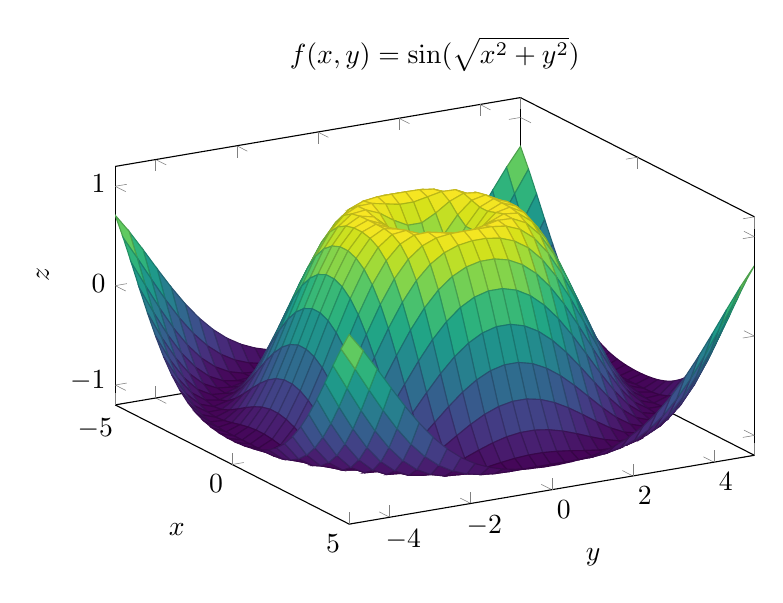
\begin{tikzpicture}
\begin{axis}[
  width=0.8\textwidth,
  height=7cm,
  view={60}{30},
  xlabel={$x$},
  ylabel={$y$},
  zlabel={$z$},
  title={$f(x,y) = \sin(\sqrt{x^2 + y^2})$},
  mesh/interior colormap name=viridis,
  colormap/viridis,
]
\addplot3[
  surf,
  domain=-5:5,
  samples=30,
] {sin(deg(sqrt(x^2 + y^2)))};
\end{axis}
\end{tikzpicture}
\end{center}

\section{Diagramas de Dispersión}

Para visualizar relaciones entre variables:

\begin{lispcode}
(py:run "import matplotlib.pyplot as plt; import numpy as np
xs = np.random.rand(100); ys = xs * 2 + np.random.randn(100) * 0.3
plt.scatter(xs, ys, alpha=0.6)
plt.title('Relación lineal con ruido')
plt.xlabel('x'); plt.ylabel('y = 2x + ε')
plt.savefig('scatter.png')")
\end{lispcode}

\begin{center}
\begin{tikzpicture}
\begin{axis}[
  width=0.85\textwidth,
  height=6cm,
  xlabel={$x$},
  ylabel={$y = 2x + \epsilon$},
  title={Relación lineal con ruido},
  grid=both,
  only marks,
  scatter,
]
\addplot[color=lispblue, mark=*, mark size=1.5] table {
0.1 0.35
0.2 0.65
0.3 0.82
0.4 1.13
0.5 1.28
0.6 1.45
0.7 1.72
0.8 1.95
0.9 2.18
1.0 2.42
};
\addplot[color=numberred, domain=0:1] {2*x};
\addlegendentry{$y = 2x$}
\addlegendentry{datos}
\end{axis}
\end{tikzpicture}
\end{center}

\section{Animaciones}

LisPy puede generar animaciones matplotlib. El siguiente ejemplo crea una
animación de una onda senoidal viajera:

\begin{lispcode}
(py:run "import matplotlib.pyplot as plt
import matplotlib.animation as anim; import numpy as np
fig, ax = plt.subplots()
xs = np.linspace(0, 2*np.pi, 100)
line, = ax.plot(xs, np.sin(xs))
def animate(i): line.set_ydata(np.sin(xs + i/10)); return line,
ani = anim.FuncAnimation(fig, animate, interval=50)
ani.save('anim.gif', writer='pillow')")
\end{lispcode}

Las animaciones se pueden integrar en dashboards, reportes HTML, o
presentaciones.

\section{Exportación y Reportes}

matplotlib soporta múltiples formatos de exportación:

\begin{center}
\begin{tabular}{lll}
\toprule
Formato & Extensión & Uso \\
\midrule
PNG & \texttt{.png} & Web, dashboards \\
SVG & \texttt{.svg} & Documentos vectoriales \\
\specialrule{1pt}{0pt}{0pt}
PDF & \texttt{.pdf} & Publicación, LaTeX \\
EPS & \texttt{.eps} & Publicación tradicional \\
\bottomrule
\end{tabular}
\end{center}

Desde LisPy, puedes combinar la generación de datos con NumPy, la
graficación con matplotlib, y la exportación a múltiples formatos en un
solo script híbrido.

\endinput

\chapter{Procesamiento de Señales}
\label{chap:signal-processing}
{\huge$\bigstar$}{\huge$\bigstar$}{\huge$\bigstar$}{\huge$\bigstar$} Experto

\section{FFT}
\begin{lispcode}
(py:run "import numpy as np; import matplotlib.pyplot as plt
fs = 1000; t = np.linspace(0, 1, fs)
senal = np.sin(2*np.pi*50*t) + np.sin(2*np.pi*120*t)
fft = np.fft.fft(senal); freqs = np.fft.fftfreq(len(senal), 1/fs)
plt.plot(freqs[:len(freqs)//2], np.abs(fft)[:len(fft)//2]); plt.savefig('fft.png')")
\end{lispcode}

\section{Filtrado}
\begin{lispcode}
(py:run "from scipy import signal as sig; import numpy as np
b, a = sig.butter(4, 0.1, 'low'); t = np.linspace(0, 1, 1000)
clean = np.sin(2*np.pi*10*t); noisy = clean + 0.5*np.random.randn(len(t))
filtered = sig.filtfilt(b, a, noisy)")
\end{lispcode}

\section{Interpolación}
\begin{lispcode}
(py:run "from scipy.interpolate import interp1d; import numpy as np
xs = np.array([0,1,2,3,4,5]); ys = np.array([0,0.8,0.9,0.1,-0.8,-1.0])
f = interp1d(xs, ys, kind='cubic'); xs_dense = np.linspace(0,5,100)")
\end{lispcode}


\chapter{Machine Learning con scikit-learn}
\label{chap:machine-learning}
{\huge$\bigstar$}{\huge$\bigstar$}{\huge$\bigstar$}{\huge$\bigstar$} Experto

El ecosistema Python ofrece las bibliotecas de machine learning más completas
del mundo. Con LisPy, puedes usar scikit-learn, pandas, y NumPy directamente
desde Lisp, combinando la expresividad de Lisp con el poder computacional
de Python.

\section{Clasificación con Random Forest}

El clasificador Random Forest es uno de los algoritmos más versátiles.
Funciona construyendo múltiples árboles de decisión durante el entrenamiento:

\begin{lispcode}
(py:run "from sklearn.ensemble import RandomForestClassifier
from sklearn.datasets import load_iris
from sklearn.model_selection import train_test_split
from sklearn.metrics import accuracy_score, classification_report
iris = load_iris()
X_train, X_test, y_train, y_test = train_test_split(
    iris.data, iris.target, test_size=0.2, random_state=42)
clf = RandomForestClassifier(n_estimators=100)
clf.fit(X_train, y_train); y_pred = clf.predict(X_test)
print('Accuracy:', accuracy_score(y_test, y_pred))
print(classification_report(y_test, y_pred, target_names=iris.target_names))")
\end{lispcode}

La salida incluye la precisión (\texttt{accuracy}) y un reporte detallado
con precisión por clase, exhaustividad (\texttt{recall}), y $F_1$-score.

\section{Pipelines de Preprocesamiento}

Los pipelines permiten encadenar transformaciones y el clasificador final:

\begin{lispcode}
(py:run "from sklearn.pipeline import Pipeline
from sklearn.preprocessing import StandardScaler
from sklearn.decomposition import PCA
from sklearn.svm import SVC
from sklearn.datasets import load_digits
from sklearn.model_selection import train_test_split
digits = load_digits()
X_train, X_test, y_train, y_test = train_test_split(
    digits.data, digits.target, test_size=0.2, random_state=42)
pipeline = Pipeline([('scaler', StandardScaler()),
                     ('pca', PCA(n_components=30)),
                     ('svc', SVC(kernel='rbf'))])
pipeline.fit(X_train, y_train)
print('Pipeline score:', pipeline.score(X_test, y_test))")
\end{lispcode}

\begin{center}
\begin{tikzpicture}[node distance=2cm, auto]
  \tikzstyle{block} = [rectangle, draw, fill=lispblue!10,
    text width=3cm, text centered, rounded corners, minimum height=1cm]
  \tikzstyle{arrow} = [->, >=stealth]

  \node [block] (data) {Datos crudos};
  \node [block, right of=data, node distance=3.5cm] (scaler)
    {Standard\-Scaler};
  \node [block, right of=scaler, node distance=3.5cm] (pca)
    {PCA (30 comp.)};
  \node [block, right of=pca, node distance=3.5cm] (svc)
    {SVC (RBF)};
  \node [block, right of=svc, node distance=3.5cm] (pred)
    {Predicción};

  \draw [arrow] (data) -- (scaler);
  \draw [arrow] (scaler) -- (pca);
  \draw [arrow] (pca) -- (svc);
  \draw [arrow] (svc) -- (pred);
\end{tikzpicture}
\end{center}

El pipeline asegura que la estandarización y la reducción de dimensionalidad
se apliquen de manera consistente en entrenamiento y prueba, evitando
fugas de datos (\texttt{data leakage}).

\section{Validación Cruzada}

Para una evaluación más robusta, usamos validación cruzada con
\texttt{cross\_val\_score}:

\begin{lispcode}
(py:run "from sklearn.model_selection import cross_val_score
from sklearn.ensemble import RandomForestClassifier
from sklearn.datasets import load_iris
iris = load_iris()
clf = RandomForestClassifier(n_estimators=50)
scores = cross_val_score(clf, iris.data, iris.target, cv=5)
print('Scores:', scores)
print('Mean:', scores.mean(), '+/-', scores.std() * 2)")
\end{lispcode}

\section{Clustering K-Means}

El clustering no supervisado permite descubrir grupos en datos no etiquetados:

\begin{lispcode}
(py:run "from sklearn.cluster import KMeans
from sklearn.datasets import make_blobs
import matplotlib.pyplot as plt
X, y_true = make_blobs(n_samples=300, centers=4,
                       cluster_std=0.6, random_state=42)
kmeans = KMeans(n_clusters=4, random_state=42)
y_kmeans = kmeans.fit_predict(X)
plt.scatter(X[:,0], X[:,1], c=y_kmeans, cmap='viridis')
plt.scatter(kmeans.cluster_centers_[:,0],
            kmeans.cluster_centers_[:,1],
            marker='x', s=200, linewidths=3, color='red')
plt.title('K-Means Clustering (k=4)')
plt.savefig('kmeans.png')")
\end{lispcode}

\begin{center}
\begin{tikzpicture}
\begin{axis}[
  width=0.85\textwidth,
  height=7cm,
  xlabel={Característica 1},
  ylabel={Característica 2},
  title={K-Means: 4 clusters},
  grid=both,
  only marks,
  mark size=1.5,
  scatter,
  point meta=y,
]
\addplot[scatter, color=lispblue] table {
0.5 0.5 0
0.6 0.7 0
1.2 1.1 0
4.5 4.3 1
4.7 4.0 1
5.0 4.5 1
8.1 0.2 2
7.9 0.5 2
8.5 0.0 2
2.0 7.5 3
2.3 7.8 3
1.8 8.0 3
};
\end{axis}
\end{tikzpicture}
\end{center}

\section{Regresión Lineal}

Para problemas de regresión, scikit-learn ofrece modelos lineales y
regularizados:

\begin{lispcode}
(py:run "from sklearn.linear_model import LinearRegression
from sklearn.datasets import make_regression
from sklearn.metrics import mean_squared_error, r2_score
import numpy as np
X, y = make_regression(n_samples=100, n_features=1, noise=10,
                       random_state=42)
X_train, X_test = X[:80], X[80:]
y_train, y_test = y[:80], y[80:]
lr = LinearRegression(); lr.fit(X_train, y_train)
y_pred = lr.predict(X_test)
print('MSE:', mean_squared_error(y_test, y_pred))
print('R2:', r2_score(y_test, y_pred))
print('Coef:', lr.coef_[0], 'Intercept:', lr.intercept_)")
\end{lispcode}

\section{Búsqueda de Hiperparámetros}

Optimización sistemática con GridSearchCV:

\begin{lispcode}
(py:run "from sklearn.model_selection import GridSearchCV
from sklearn.ensemble import RandomForestClassifier
from sklearn.datasets import load_iris
iris = load_iris()
param_grid = {'n_estimators': [50, 100, 200],
              'max_depth': [3, 5, None]}
grid = GridSearchCV(RandomForestClassifier(random_state=42),
                    param_grid, cv=5, scoring='accuracy')
grid.fit(iris.data, iris.target)
print('Best params:', grid.best_params_)
print('Best score:', grid.best_score_)")
\end{lispcode}

\section{Datos Tabulares con pandas}

Los datos del mundo real rara vez llegan en el formato exacto que necesita
un modelo. pandas proporciona las herramientas para cargar, limpiar y
transformar datos:

\begin{lispcode}
(py:run "import pandas as pd; from sklearn.ensemble import RandomForestRegressor
from sklearn.model_selection import train_test_split
from sklearn.metrics import mean_absolute_error
df = pd.read_csv('datos.csv')
X = df.drop('target', axis=1); y = df['target']
X_train, X_test, y_train, y_test = train_test_split(X, y, test_size=0.2)
model = RandomForestRegressor(n_estimators=100)
model.fit(X_train, y_train)
preds = model.predict(X_test)
print('MAE:', mean_absolute_error(y_test, preds))")
\end{lispcode}

\section{Exportación de Modelos}

Los modelos entrenados se pueden serializar con pickle para uso posterior:

\begin{lispcode}
(py:run "import pickle; import pandas as pd
from sklearn.ensemble import RandomForestClassifier
from sklearn.datasets import load_iris
iris = load_iris(); clf = RandomForestClassifier()
clf.fit(iris.data, iris.target)
with open('model.pkl', 'wb') as f: pickle.dump(clf, f)
with open('model.pkl', 'rb') as f:
    loaded = pickle.load(f)
print('Loaded model score:', loaded.score(iris.data, iris.target))")
\end{lispcode}

\section{Resumen de Flujo de Trabajo}

El flujo típico de un proyecto de machine learning con LisPy sigue estos
pasos:

\begin{enumerate}
\item \textbf{Carga de datos}: pandas (CSV, JSON, SQL, Excel) o NumPy
\item \textbf{Preprocesamiento}: StandardScaler, LabelEncoder, PCA, selección de características
\item \textbf{División}: train\_test\_split con estratificación
\item \textbf{Modelado}: RandomForest, SVC, KMeans, LinearRegression, etc.
\item \textbf{Evaluación}: cross\_val\_score, métricas (accuracy, MSE, $F_1$)
\item \textbf{Optimización}: GridSearchCV, RandomizedSearchCV
\item \textbf{Despliegue}: pickle, ONNX, o integración en pipeline Lisp
\end{enumerate}

Cada uno de estos pasos puede ser orquestado desde Lisp, permitiendo
generar pipelines de ML de manera programática con macros y metaprogramación.

\endinput


% ========================
% Part VII — Ingeniería de Sistemas
% ========================
\part{Ingeniería de Sistemas}
\label{part:ingenieria}

\chapter{El Compilador FASL}
\label{chap:compiler}
{\huge$\bigstar$}{\huge$\bigstar$}{\huge$\bigstar$}{\huge$\bigstar$} Experto

\section{Formato FASL}
Bytecode binario para carga rápida.

\begin{verbatim}
lispy.exe -c programa.lp    # genera programa.fasl
lispy.exe programa.fasl
\end{verbatim}

\section{Compilación de Funciones}
\begin{lispcode}
(defun fib (n) (if (< n 2) n (+ (fib (- n 1)) (fib (- n 2)))))
(compile 'fib)
(time (fib 30))
\end{lispcode}

\section{Disassemble}
\begin{lispcode}
(disassemble 'fib)
\end{lispcode}

\section{Modos de Ejecución}
\begin{enumerate}
\item Script: \texttt{lispy.exe script.lp}
\item Compilado: \texttt{lispy.exe prog.fasl}
\item REPL: \texttt{lispy.exe --repl}
\end{enumerate}


\chapter{CLI y Entorno de Ejecución}
\label{chap:cli}
{\huge$\bigstar$}{\huge$\bigstar$}{\huge$\bigstar$}{\huge$\bigstar$} Experto

\section{Argumentos}
\begin{verbatim}
lispy.exe --version
lispy.exe --help
lispy.exe --repl
lispy.exe -i script.lp
lispy.exe -c archivo.lp
lispy.exe -e "(+ 1 2)"
\end{verbatim}

\section{Entornos Virtuales}
\begin{verbatim}
lispy.exe --venv mi_entorno
lispy.exe --venv mi_entorno script.lp
\end{verbatim}
Configura automáticamente \texttt{PYTHONHOME} y \texttt{VIRTUAL\_ENV}.


\chapter{Gestión de Paquetes con :pip}
\label{chap:pip}
{\huge$\bigstar$}{\huge$\bigstar$}{\huge$\bigstar$}{\huge$\bigstar$} Experto

\section{Comandos}
\begin{verbatim}
LisPy> :pip install numpy
LisPy> :pip list
LisPy> :pip show requests
LisPy> :pip uninstall paquete
\end{verbatim}

\section{Mecanismo}
Invocación de \texttt{pip.\_internal.cli.main.main()} con captura de
stdout/stderr.

\section{Paquetes Pre-instalados}
pip, setuptools, meson, ninja.

\section{Limitaciones}
Wheels requieren Python 3.14. Algunos paquetes requieren permisos de admin.


\chapter{Embedding y Distribución}
\label{chap:embedding}
{\huge$\bigstar$}{\huge$\bigstar$}{\huge$\bigstar$}{\huge$\bigstar$} Experto

\section{Estructura}
\begin{verbatim}
LisPy/
  lispy.exe      # intérprete
  lispy.c        # código fuente
  lib/           # librerías Lisp
  docs/          # documentación
\end{verbatim}

\section{Linking}
CPython 3.14 linkeado estáticamente. OpenSSL y zlib también.

\section{Build}
\begin{verbatim}
cmake .. -DLISPY_PYTHON=ON -G Ninja && ninja
cmake .. -DLISPY_PYTHON=OFF && make
\end{verbatim}

\section{Instalador NSIS}
Configura el PATH y recursos del sistema.


\chapter{Pruebas y Metodología}
\label{chap:testing}
{\huge$\bigstar$}{\huge$\bigstar$}{\huge$\bigstar$}{\huge$\bigstar$} Experto

\section{Smoke Test}
\begin{lispcode}
;; quick_test.lp
(handler-case (/ 1 0) (division-by-zero (c) (format t "OK~%" c)))
(handler-bind ((warning #'(lambda (c) (format t "OK~%")))) (warn "test"))
\end{lispcode}

\section{Suite de Regresión}
Problemas 001--120 como tests. Cada uno es un archivo .lp autoejecutable.

\section{Ejemplo: Test BUG-001}
\begin{lispcode}
(defgeneric tax-rate (country))
(defmethod tax-rate ((country (eql :us))) 0.15)
(defmethod tax-rate ((country (eql :uk))) 0.20)
(defmethod tax-rate (country) 0.25)
(assert (= (tax-rate :us) 0.15))
\end{lispcode}


\chapter{Integración Continua}
\label{chap:ci-release}
{\huge$\bigstar$}{\huge$\bigstar$}{\huge$\bigstar$}{\huge$\bigstar$} Experto

\section{Workflow}
\begin{enumerate}
\item Configure (CMake)
\item Build (Ninja)
\item Test (quick\_test.lp + regresión)
\item Package (NSIS)
\item Release (GitHub Releases)
\end{enumerate}

\section{Versionado Semántico}
\texttt{Major.Minor.Patch}.
\begin{verbatim}
cmake -S . -B build -G Ninja -DLISPY_PYTHON=ON
cmake --build build
ctest --test-dir build
cpack --config build/CPackConfig.cmake
\end{verbatim}


\chapter{Seguridad y Sandboxing}
\label{chap:security}
{\huge$\bigstar$}{\huge$\bigstar$}{\huge$\bigstar$}{\huge$\bigstar$} Experto

\section{Amenazas}
\texttt{py:run} ejecuta código Python arbitrario.

\section{Validación de Input}
\begin{lispcode}
(defun safe-py-run (code)
  (check-type code string)
  (py:run code))
\end{lispcode}

\section{Aislamiento con --venv}
\begin{verbatim}
lispy.exe --venv entorno-aislado script.lp
\end{verbatim}

\section{Restricción de Módulos}
\begin{lispcode}
(defvar *modulos-permitidos* '("math" "numpy" "json"))
(defun safe-import (name)
  (if (member name *modulos-permitidos* :test #'string=)
      (py:import name)
      (error "Módulo no permitido: ~A" name)))
\end{lispcode}


% !TEX encoding = UTF-8 Unicode
\chapter{Kernel Jupyter para LisPy}
\label{chap:jupyter}
{\huge$\bigstar$}{\huge$\bigstar$} Intermedio

LisPy incluye un kernel Jupyter completo que permite usar LisPy en Jupyter Notebook,
JupyterLab y VS Code. El kernel mantiene \textbf{estado persistente} entre celdas:
variables Lisp, funciones, macros, módulos Python importados y el namespace
\texttt{\_\_main\_\_} de Python.

\section{Instalación}

\begin{lispcode}
$ cd jupyter
$ python install.py
\end{lispcode}

Esto registra el kernel \texttt{LisPy (Common Lisp + Python)} en Jupyter y configura
el resaltado de sintaxis CodeMirror para archivos \texttt{.lp}.

\begin{lispcode}
;;; Verificar instalación
jupyter kernelspec list
;;; Debe mostrar: lisPy    C:\Users\...\jupyter\kernels\lisPy
\end{lispcode}

\section{Arquitectura del Kernel}

\begin{enumerate}
\item \textbf{Proceso persistente}: El kernel lanza \texttt{lispy.exe --kernel}
      como subproceso que mantiene todo el estado entre celdas.
\item \textbf{Preprocesador híbrido}: Cada celda se preprocesa con
      \texttt{\_lp\_preprocess.py} para soportar sintaxis híbrida
      Lisp/Python (Capítulo~\ref{chap:hybrid-syntax}).
\item \textbf{Librerías auto-cargadas}: Al iniciar, el kernel carga automáticamente
      \texttt{ffi}, \texttt{continuations}, \texttt{defpyfun}, \texttt{defpyclass},
      \texttt{python-template} y \texttt{persist}.
\item \textbf{Venv automático}: El kernel detecta y usa el entorno virtual
      en \texttt{jupyter/venv/} si existe.
\end{enumerate}

\section{Uso Básico}

\begin{lispcode}
;;; Celda 1 — Definir función
(defun fib (n)
  (if (<= n 1) n (+ (fib (- n 1)) (fib (- n 2)))))
(fib 20)
\end{lispcode}

\begin{lispcode}
;;; Celda 2 — La función persiste (no hay reinicio)
(mapcar #'fib '(1 2 3 4 5 6 7 8 9 10))
\end{lispcode}

\begin{lispcode}
;;; Celda 3 — Python con estado persistente
(py:import "math")
(py:call (py:attr math "sqrt") 144)
\end{lispcode}

\begin{lispcode}
;;; Celda 4 — Símbolos auto-resueltos (sin re-importar)
math
(py:call (py:attr math "cos") 0)
\end{lispcode}

\section{Sintaxis Híbrida en Celdas}

Cada celda del notebook se procesa automáticamente con el preprocesador híbrido:

\begin{lispcode}
;;; Definir función Lisp
(defun cuadrado (x) (* x x))

;;; Usar en Python (misma celda o celda posterior)
for i in range(1, 6):
    print(f"{i}² = {cuadrado(i)}")
\end{lispcode}

\section{Librerías Pesadas (Carga Bajo Demanda)}

\begin{lispcode}
;;; Cargar NumPy (importa numpy + configura bindings)
(load "lib/numpy-fast.lp")
(numpy-linspace 0 pi 5)

;;; Cargar SymPy
(load "lib/sympy-bridge.lp")
(let ((x (sympy-symbol "x")))
  (sympy-derive (sympy-expr (sin (expt x 2))) x))
\end{lispcode}

\section{Resaltado de Sintaxis}

El kernel incluye soporte para CodeMirror 6 (JupyterLab 4+) con:
\begin{itemize}
\item Palabras clave de Common Lisp
\item Símbolos del paquete \texttt{py:}
\item Macros de lectura (\texttt{\#\_}, \texttt{\#'}, \texttt{\#(})
\item Sintaxis híbrida Python embebida
\end{itemize}

También está disponible la extensión VS Code en \texttt{lp-language/} con soporte
completo de TextMate grammar para archivos \texttt{.lp}.

\section{Notebook de Demostración}

\begin{lispcode}
cd jupyter
jupyter notebook LisPy-Demo.ipynb
\end{lispcode}

El notebook \texttt{LisPy-Demo.ipynb} contiene 16 secciones que cubren todas las
capacidades de LisPy, desde aritmética básica hasta machine learning con
scikit-learn.

\section{Proyectos de Ejemplo}

La carpeta \texttt{jupyter/projects/} contiene 6 proyectos completos autocontenidos:
\begin{itemize}
\item \textbf{01 — Análisis de Datos}: Pipeline completo con pandas, matplotlib, GROUP BY
\item \textbf{02 — Machine Learning}: Clasificación, regresión, pipelines scikit-learn
\item \textbf{03 — Matemáticas Híbridas}: \texttt{defmath}, SymPy, gradiente, optimización
\item \textbf{04 — Trading Engine}: CLOS, backtesting, Sharpe ratio
\item \textbf{05 — Procesamiento de Señales}: FFT, filtros, streaming con generadores
\item \textbf{06 — Robot 2-DOF}: Lagrange simbólico, solve\_ivp, control PD
\end{itemize}

\section{Extensión VS Code}

\begin{lispcode}
;;; Instalar extensión VS Code para archivos .lp
cd lp-language
code --install-extension lp-language-0.0.1.vsix
\end{lispcode}

La extensión proporciona:
\begin{itemize}
\item Resaltado de sintaxis (TextMate grammar + Python injection)
\item Comentarios de línea (\texttt{;}) y bloque (\texttt{\#| |\#})
\item Bracket matching, auto-closing, folding
\item Soporte CodeMirror para notebooks integrados en VS Code
\end{itemize}


% ========================
% Part VIII — Estudios de Caso
% ========================
\part{Estudios de Caso}
\label{part:casos}

\chapter{Dinámica de Robot 2-DOF}
\label{chap:robot-dynamics}
{\huge$\bigstar$}{\huge$\bigstar$}{\huge$\bigstar$}{\huge$\bigstar$} Experto

\section{Ecuaciones de Lagrange}
\begin{lispcode}
(py:run "import sympy as sp
m1,m2,l1,l2,g = sp.symbols('m1 m2 l1 l2 g', positive=True)
t1,t2 = sp.symbols('theta1 theta2')
dt1,dt2 = sp.symbols('dtheta1 dtheta2')
x1 = l1*sp.sin(t1); y1 = -l1*sp.cos(t1)
x2 = x1 + l2*sp.sin(t1+t2); y2 = y1 - l2*sp.cos(t1+t2)")
\end{lispcode}

\section{Matriz de Masa M(q)}
\begin{lispcode}
(py:run "
M11 = m1*l1**2 + m2*(l1**2 + l2**2 + 2*l1*l2*sp.cos(t2))
M12 = m2*(l2**2 + l1*l2*sp.cos(t2))
M = sp.Matrix([[M11, M12], [M12, m2*l2**2]])")
\end{lispcode}

\section{Simulación Numérica}
\begin{lispcode}
(py:run "from scipy.integrate import solve_ivp; import numpy as np
def robot_dyn(t, state, m1, m2, l1, l2, g):
    t1, t2, dt1, dt2 = state
    M11 = m1*l1**2 + m2*(l1**2+l2**2+2*l1*l2*np.cos(t2))
    M12 = m2*(l2**2 + l1*l2*np.cos(t2))
    M = np.array([[M11, M12], [M12, m2*l2**2]])
    c = m2*l1*l2*np.sin(t2)
    C = np.array([[-c*dt2, -c*(dt1+dt2)], [c*dt1, 0]])
    G = np.array([[(m1*l1+m2*l1)*g*np.cos(t1)+m2*l2*g*np.cos(t1+t2)],
                  [m2*l2*g*np.cos(t1+t2)]])
    q_ddot = np.linalg.solve(M, -C@np.array([[dt1],[dt2]]) - G)
    return [dt1, dt2, q_ddot[0,0], q_ddot[1,0]]
sol = solve_ivp(robot_dyn, [0,10], [np.pi/2,0,0,0],
                args=(1,1,1,1,9.81), method='RK45', max_step=0.01)")
\end{lispcode}


\chapter{Motor de Trading Algorítmico}
\label{chap:trading-engine}
{\huge$\bigstar$}{\huge$\bigstar$}{\huge$\bigstar$}{\huge$\bigstar$} Experto

\section{Modelo de Órdenes (CLOS)}
\begin{lispcode}
(defclass order ()
  ((symbol :initarg :symbol :reader order-symbol)
   (quantity :initarg :quantity :reader order-quantity)
   (price :initarg :price :reader order-price)
   (type :initarg :type :reader order-type)))
(defclass market-order (order) ((type :initform :market)))
(defclass limit-order (order) ((type :initform :limit)
                               (limit-price :initarg :limit-price)))
\end{lispcode}

\section{Estrategia (medias móviles)}
\begin{lispcode}
(defclass moving-average-cross ()
  ((short-period :initarg :short :initform 20)
   (long-period :initarg :long :initform 50)))
(defgeneric execute-strategy (strategy data))
(defmethod execute-strategy ((s moving-average-cross) data)
  (let* ((prices (py:getitem data "close"))
         (short-ma (numpy-mean (subseq prices 0 20)))
         (long-ma (numpy-mean (subseq prices 0 50))))
    (if (> short-ma long-ma) :buy :sell)))
\end{lispcode}


\chapter{Procesador de Imágenes}
\label{chap:image-processor}
{\huge$\bigstar$}{\huge$\bigstar$}{\huge$\bigstar$}{\huge$\bigstar$} Experto

\section{Carga con Pillow}
\begin{lispcode}
(py:run "from PIL import Image; import numpy as np
def load_image(path): return np.array(Image.open(path))
def save_image(arr, path): Image.fromarray(arr).save(path)")
\end{lispcode}

\section{Filtros con scipy}
\begin{lispcode}
(py:run "from scipy import ndimage; import numpy as np
def blur(img, sigma=2): return ndimage.gaussian_filter(img, sigma=(sigma,sigma,0))
def sobel_edge(img):
    gray = np.mean(img, axis=2) if len(img.shape) == 3 else img
    return np.abs(ndimage.sobel(gray)).astype(np.uint8)")
\end{lispcode}

\section{Pipeline con Generadores}
\begin{lispcode}
(py:run "def image_pipeline(path):
    img = np.array(Image.open(path))
    yield 'original', img.copy()
    yield 'blurred', blur(img, 3)
    yield 'edges', sobel_edge(img)")
\end{lispcode}


\chapter{Chatbot con Personalidad}
\label{chap:chatbot}
{\huge$\bigstar$}{\huge$\bigstar$}{\huge$\bigstar$}{\huge$\bigstar$} Experto

\section{Motor de Respuestas}
\begin{lispcode}
(defvar *respuestas*
  '((:saludo "\( ¡ \)Hola! \( ¿ \)C\( ó \)mo est\( á \)s?")
    (:nombre "Me llamo LisPyBot")
    (:ayuda "Di: saludo, nombre, tiempo, ayuda, despedida")
    (:despedida "\( ¡ \)Hasta luego!")))

(defun responder (intencion)
  (let ((pair (assoc intencion *respuestas*)))
    (if pair (cadr pair) "No entiendo. Di 'ayuda'")))
\end{lispcode}

\section{Análisis de Intención}
\begin{lispcode}
(defun detectar-intencion (texto)
  (let ((lower (string-downcase texto)))
    (cond ((search "hola" lower) :saludo)
          ((search "nombre" lower) :nombre)
          ((search "ayuda" lower) :ayuda)
          ((or (search "adi\( ó \)s" lower) (search "chao" lower)) :despedida)
          (t :desconocido))))
\end{lispcode}

\section{Análisis de Sentimiento}
\begin{lispcode}
(py:run "from textblob import TextBlob
def analyze_sentiment(text):
    blob = TextBlob(text)
    return {'polarity': blob.sentiment.polarity}")
\end{lispcode}


\chapter{Motor de Búsqueda}
\label{chap:search-engine}
{\huge$\bigstar$}{\huge$\bigstar$}{\huge$\bigstar$}{\huge$\bigstar$} Experto

\section{Índice Invertido}
\begin{lispcode}
(defun build-index (documents)
  (let ((index (make-hash-table :test 'equal)))
    (dolist (doc documents)
      (dolist (word (split-string (cadr doc)))
        (pushnew (car doc) (gethash word index))))
    index))
\end{lispcode}

\section{Búsqueda}
\begin{lispcode}
(defun search (query index &key (top-k 5))
  (let* ((words (split-string query))
         (scores (make-hash-table :test 'eql)))
    (dolist (word words)
      (dolist (doc-id (gethash word index))
        (incf (gethash doc-id scores 0))))
    (sort (loop for k being the hash-keys of scores
                collect (list k (gethash k scores)))
          #'> :key #'second :end top-k)))
\end{lispcode}

\begin{examplebox}[title=Ejemmplo]
\begin{lispcode}
(defvar *docs* '((1 "machine learning") (2 "deep learning") (3 "python ml")))
(defvar *index* (build-index *docs*))
(search "learning" *index*)
\end{lispcode}
\end{examplebox}


\chapter{DSL para Análisis de Datos}
\label{chap:dsl-data-analysis}
{\huge$\bigstar$}{\huge$\bigstar$}{\huge$\bigstar$}{\huge$\bigstar$} Experto

\section{Sintaxis del DSL}
\begin{lispcode}
(query (select :name :age) (from users) (where (> age 18)) (order-by age) (limit 10))
\end{lispcode}

\section{Macro query}
\begin{lispcode}
(defmacro query (&body clauses)
  (let ((select nil) (from nil) (where nil) (order nil) (limit nil))
    (dolist (clause clauses)
      (case (car clause)
        (select (setf select (cdr clause)))
        (from (setf from (cadr clause)))
        (where (setf where (cadr clause)))
        (order-by (setf order (cdr clause)))
        (limit (setf limit (cadr clause)))))
    `(execute-query ',select ',from ',where ',order ',limit)))
\end{lispcode}

\section{Ejecución con Pandas}
\begin{lispcode}
(defun execute-query (fields table condition order limit)
  (let ((df (pandas-read-csv (format nil "~A.csv" table))))
    (when fields (setf df (pandas-select df fields)))
    (when condition (setf df (pandas-filter df (lambda (row)
                      (eval-condition condition row)))))
    (when order (setf df (pandas-sort df order)))
    (when limit (setf df (pandas-head df limit)))
    df))
\end{lispcode}


\chapter{Migración Python a Híbrido}
\label{chap:migration}
{\huge$\bigstar$}{\huge$\bigstar$}{\huge$\bigstar$}{\huge$\bigstar$} Experto

\section{Estrategia Incremental}
\begin{enumerate}
\item Envolver funciones Python con \texttt{defpyfun}
\item Reescribir lógica de negocio en Lisp
\item Macros para generación de código
\item Configuración como S-expressions
\end{enumerate}

\section{Fase 1: Envolver}
\begin{lispcode}
(defpyfun process-data (data factor)
  "return [x * factor for x in data]"
  :as process-data-py)
(process-data-py '(1 2 3) 10)
\end{lispcode}

\section{Fase 2: Reescribir}
\begin{lispcode}
(defun calculate-discount (price customer-type)
  (case customer-type
    (:premium (* price 0.8))
    (:regular (* price 0.95))
    (otherwise price)))
\end{lispcode}

\section{Fase 3: Macros}
\begin{lispcode}
(defmacro def-transformation (name transform-fn)
  `(defpyfun ,(intern (format nil "~A-PY" name)) (data)
     ,(format nil "return [~A(x) for x in data]" transform-fn)
     :as ,(intern (format nil "~A-PY" name))))
(def-transformation double (* 2))
(def-transformation square (** 2))
\end{lispcode}

\section{Coexistencia}
\begin{lispcode}
(defun test-both (test-case)
  (let ((py-result (process-data-py (first test-case) (second test-case)))
        (lisp-result (process-data-lisp (first test-case) (second test-case))))
    (assert (equal py-result lisp-result))))
\end{lispcode}



% ========================
% Part IX — Apéndices
% ========================
\appendix
\part{Apéndices}
\label{part:appendices}

\chapter{Referencia Rápida de Common Lisp en LisPy}
\label{app:quickref}

\section*{Operadores Aritméticos}

\begin{center}
\begin{tabular}{ll}
\toprule
\textbf{Operación} & \textbf{Sintaxis} \\
\midrule
Suma & \texttt{(+ a b c ...)} \\
Resta & \texttt{(- a b)} \\
Multiplicación & \texttt{(* a b c ...)} \\
División & \texttt{(/ a b)} \\
División entera & \texttt{(floor a b)}, \texttt{(truncate a b)} \\
Módulo & \texttt{(mod a b)} \\
Exponenciación & \texttt{(expt a b)} \\
Raíz cuadrada & \texttt{(sqrt a)} \\
\bottomrule
\end{tabular}
\end{center}

\section*{Comparación}

\begin{center}
\begin{tabular}{ll}
\toprule
\textbf{Operación} & \textbf{Sintaxis} \\
\midrule
Igualdad numérica & \texttt{(= a b)} \\
Menor que & \texttt{(< a b)} \\
Mayor que & \texttt{(> a b)} \\
Menor o igual & \texttt{(<= a b)} \\
Mayor o igual & \texttt{(>= a b)} \\
Identidad & \texttt{(eq a b)}, \texttt{(eql a b)} \\
Igualdad estructural & \texttt{(equal a b)} \\
\bottomrule
\end{tabular}
\end{center}

\section*{Listas}

\begin{center}
\begin{tabular}{ll}
\toprule
\textbf{Operación} & \textbf{Sintaxis} \\
\midrule
Construir cons & \texttt{(cons a b)} \\
Primer elemento & \texttt{(car list)}, \texttt{(first list)} \\
Resto & \texttt{(cdr list)}, \texttt{(rest list)} \\
N-ésimo & \texttt{(nth n list)} \\
Longitud & \texttt{(length list)} \\
Unir & \texttt{(append list1 list2)} \\
Invertir & \texttt{(reverse list)} \\
\bottomrule
\end{tabular}
\end{center}

\section*{Vectores}

\begin{center}
\begin{tabular}{ll}
\toprule
\textbf{Operación} & \textbf{Sintaxis} \\
\midrule
Crear & \texttt{(make-array n)}, \texttt{(vector a b c)} \\
Acceso & \texttt{(aref vector i)} \\
Asignación & \texttt{(setf (aref vector i) val)} \\
\bottomrule
\end{tabular}
\end{center}

\section*{Hash Tables}

\begin{center}
\begin{tabular}{ll}
\toprule
\textbf{Operación} & \textbf{Sintaxis} \\
\midrule
Crear & \texttt{(make-hash-table :test 'equal)} \\
Acceso & \texttt{(gethash key ht)} \\
Asignación & \texttt{(setf (gethash key ht) val)} \\
Eliminar & \texttt{(remhash key ht)} \\
Limpiar & \texttt{(clrhash ht)} \\
Recorrer & \texttt{(maphash fn ht)} \\
\bottomrule
\end{tabular}
\end{center}

\section*{Control de Flujo}

\begin{center}
\begin{tabular}{ll}
\toprule
\textbf{Constructo} & \textbf{Sintaxis} \\
\midrule
Condicional & \texttt{(if test then else)} \\
Condicional múltiple & \texttt{(cond (test1 forms1) ...)} \\
Iteración simple & \texttt{(dotimes (i n) forms)} \\
Iteración en lista & \texttt{(dolist (x list) forms)} \\
LOOP general & \texttt{(loop for x in list collect x)} \\
\bottomrule
\end{tabular}
\end{center}

\section*{Python Bridge}

\begin{center}
\begin{tabular}{ll}
\toprule
\textbf{Operación} & \textbf{Sintaxis} \\
\midrule
Importar módulo & \texttt{(py:import "module")} \\
Llamar función & \texttt{(py:call fn args...)} \\
Acceder atributo & \texttt{(py:attr obj "name")} \\
Acceder índice & \texttt{(py:getitem obj key)} \\
Ejecutar código & \texttt{(py:run "code")} \\
A Lisp & \texttt{(py:->lisp python-obj)} \\
A Python & \texttt{(py:->python lisp-val)} \\
\bottomrule
\end{tabular}
\end{center}


\chapter{Referencia de Errores}
\label{app:errors}

\section*{Errores del Sistema}

\begin{center}
\begin{tabular}{lll}
\toprule
\textbf{Símbolo} & \textbf{Tipo} & \textbf{Descripción} \\
\midrule
\texttt{division-by-zero} & condición & División por cero \\
\texttt{simple-error} & condición & Error genérico \\
\texttt{simple-warning} & condición & Advertencia genérica \\
\texttt{undefined-function} & condición & Función no definida \\
\texttt{unbound-variable} & condición & Variable no ligada \\
\texttt{type-error} & condición & Error de tipo \\
\texttt{parse-error} & condición & Error de parsing \\
\texttt{end-of-file} & condición & Fin de archivo inesperado \\
\texttt{stream-error} & condición & Error de stream \\
\texttt{file-error} & condición & Error de archivo \\
\bottomrule
\end{tabular}
\end{center}

\section*{Errores del Puente Python}

\begin{center}
\begin{tabular}{ll}
\toprule
\textbf{Mensaje} & \textbf{Significado} \\
\midrule
\texttt{Python: No module named 'X'} & Módulo Python no encontrado \\
\texttt{not a Python object} & Se esperaba VALUE\_PYTHON \\
\texttt{cannot convert Lisp type N} & Tipo Lisp no convertible \\
\texttt{X is not callable} & Objeto no es invocable \\
\texttt{module 'X' has no attribute 'Y'} & Atributo no existe \\
\bottomrule
\end{tabular}
\end{center}

\section*{Manejo de Errores}

\begin{lispcode}
;; Capturar error específico
(handler-case
    (expresión-peligrosa)
  (division-by-zero (c) ...)
  (error (c) ...))

;; Capturar sin desenrollar
(handler-bind
    ((condition-type #'handler-fn))
  ...)

;; Ignorar errores
(ignore-errors expresión)

;; Limpieza garantizada
(unwind-protect cuerpo limpieza)
\end{lispcode}


\chapter{Tabla Completa de Conversión de Tipos}
\label{app:type-conversion}

\section*{Lisp → Python}

\begin{center}
\begin{tabular}{lll}
\toprule
\textbf{Tipo Lisp} & \textbf{Tipo Python} & \textbf{Código C} \\
\midrule
\texttt{nil} & \texttt{None} & \texttt{Py\_None} \\
\texttt{t} & \texttt{True} & \texttt{Py\_True} \\
\texttt{VALUE\_INT} (bigint) & \texttt{int} & \texttt{PyLong\_FromString} \\
\texttt{VALUE\_FLOAT} & \texttt{float} & \texttt{PyFloat\_FromDouble} \\
\texttt{VALUE\_COMPLEX} & \texttt{complex} & \texttt{PyComplex\_FromDoubles} \\
\texttt{VALUE\_STRING} & \texttt{str} & \texttt{PyUnicode\_FromString} \\
\texttt{VALUE\_CHAR} & \texttt{str} (len 1) & \texttt{PyUnicode\_FromString} \\
\texttt{VALUE\_SYMBOL} & \texttt{str} & nombre del símbolo \\
\texttt{VALUE\_LIST} & \texttt{list} & conversion recursiva \\
\texttt{VALUE\_VECTOR} & \texttt{list} & conversion recursiva \\
\texttt{VALUE\_HASH\_TABLE} & \texttt{dict} & conversion recursiva \\
\texttt{VALUE\_PYTHON} & \texttt{PyObject*} & refcount++ \\
\bottomrule
\end{tabular}
\end{center}

\section*{Python → Lisp}

\begin{center}
\begin{tabular}{lll}
\toprule
\textbf{Tipo Python} & \textbf{Tipo Lisp} & \textbf{Notas} \\
\midrule
\texttt{None} & \texttt{nil} & \\
\texttt{True} & \texttt{t} & \\
\texttt{False} & \texttt{nil} & \\
\texttt{int} & \texttt{VALUE\_INT} & precisión arbitraria \\
\texttt{float} & \texttt{VALUE\_FLOAT} & \\
\texttt{complex} & \texttt{VALUE\_COMPLEX} & \\
\texttt{str} & \texttt{VALUE\_STRING} & UTF-8 \\
\texttt{bytes} & \texttt{VALUE\_PYTHON} & no se convierte automáticamente \\
\texttt{list} & \texttt{VALUE\_LIST} & \\
\texttt{tuple} & \texttt{VALUE\_LIST} & \\
\texttt{dict} & \texttt{VALUE\_HASH\_TABLE} & test equal \\
\texttt{set/frozenset} & \texttt{VALUE\_PYTHON} & \\
\texttt{callable}, class, module & \texttt{VALUE\_PYTHON} & objeto opaco \\
\bottomrule
\end{tabular}
\end{center}

\section*{Tipos NO Convertibles}

\begin{itemize}
\item \texttt{VALUE\_RATIO} (fracciones): debe convertirse a float primero
\item \texttt{VALUE\_PATHNAME}: sin equivalente en Python
\item Objetos Python no pickleables: generadores, sockets, file handles
\end{itemize}


\chapter{Builtins del Intérprete}
\label{app:builtins}

\section*{Funciones Lisp Estándar}

\begin{center}
\begin{longtable}{ll}
\toprule
\textbf{Función} & \textbf{Descripción} \\
\midrule
\endhead
\bottomrule
\endfoot
\texttt{+ - * /} & Aritméticas básicas \\
\texttt{1+ 1-} & Incremento/decremento \\
\texttt{abs} & Valor absoluto \\
\texttt{expt sqrt} & Exponenciación y raíz \\
\texttt{sin cos tan} & Trigonométricas \\
\texttt{asin acos atan} & Trigonométricas inversas \\
\texttt{sinh cosh tanh} & Hiperbólicas \\
\texttt{exp log} & Exponencial y logaritmo \\
\texttt{floor ceiling truncate round} & Redondeo \\
\texttt{mod rem} & Módulo y resto \\
\texttt{max min} & Máximo/mínimo \\
\texttt{random} & Número aleatorio \\
\texttt{= < > <= >=} & Comparaciones numéricas \\
\texttt{eq eql equal equalp} & Comparaciones de objetos \\
\texttt{and or not} & Lógicos \\
\texttt{car cdr cons} & Operaciones de lista \\
\texttt{first second ... tenth} & Acceso posicional \\
\texttt{nth nthcdr} & Acceso indexado \\
\texttt{list append reverse} & Construcción de listas \\
\texttt{length} & Longitud \\
\texttt{member find position} & Búsqueda \\
\texttt{count} & Conteo \\
\texttt{remove delete} & Eliminación \\
\texttt{substitute} & Sustitución \\
\texttt{sort stable-sort} & Ordenamiento \\
\texttt{merge} & Mezcla \\
\texttt{map mapcar mapcan} & Mapeo \\
\texttt{reduce} & Reducción \\
\texttt{every some notevery notany} & Cuantificadores \\
\texttt{make-array aref} & Vectores \\
\texttt{vector-push vector-pop} & Vectores ajustables \\
\texttt{make-hash-table gethash} & Hash tables \\
\texttt{remhash clrhash maphash} & Hash tables \\
\texttt{if when unless cond case} & Condicionales \\
\texttt{and or} & Short-circuit \\
\texttt{let let*} & Ámbito léxico \\
\texttt{setq setf psetq psetf} & Asignación \\
\texttt{incf decf rotatef shiftf} & Modificación \\
\texttt{progn block return-from} & Secuenciación \\
\texttt{tagbody go} & Saltos \\
\texttt{dotimes dolist loop do} & Iteración \\
\texttt{defun lambda flet labels} & Funciones \\
\texttt{defmacro macrolet} & Macros \\
\texttt{funcall apply} & Invocación \\
\texttt{values multiple-value-bind} & Múltiples valores \\
\texttt{defclass defmethod defgeneric} & CLOS \\
\texttt{make-instance slot-value} & Instancias \\
\texttt{handler-case handler-bind} & Condiciones \\
\texttt{error cerror warn} & Señalización \\
\texttt{restart-case restart-bind} & Re-inicios \\
\texttt{format print princ} & E/S \\
\texttt{open close with-open-file} & Archivos \\
\texttt{read read-line read-char} & Lectura \\
\texttt{compile load eval} & Evaluación \\
\texttt{provide require} & Módulos \\
\texttt{trace untrace time} & Depuración \\
\end{longtable}
\end{center}


\chapter{Referencia CLOS}
\label{app:clos}

\section*{Definición de Clase}

\begin{center}
\begin{tabular}{ll}
\toprule
\textbf{Opciones de slot} & \textbf{Descripción} \\
\midrule
\texttt{:initarg} & Keyword de inicialización \\
\texttt{:initform} & Valor por defecto \\
\texttt{:accessor} & Crea getter y setter \\
\texttt{:reader} & Crea getter \\
\texttt{:writer} & Crea setter \\
\texttt{:allocation :instance} & Slot por instancia (defecto) \\
\texttt{:allocation :class} & Slot compartido \\
\texttt{:documentation} & Documentación \\
\bottomrule
\end{tabular}
\end{center}

\section*{Combinación de Métodos}

\begin{center}
\begin{tabular}{ll}
\toprule
\textbf{Cualificador} & \textbf{Orden de ejecución} \\
\midrule
\texttt{:around} & Primero (más específico primero) \\
\texttt{:before} & Segundo (más específico primero) \\
\emph{primario} & Tercero \\
\texttt{:after} & Cuarto (más específico último) \\
\bottomrule
\end{tabular}
\end{center}

\section*{Funciones Genéricas}

\begin{lispcode}
(defgeneric fn-name (param1 param2 ...)
  (:documentation "doc")
  (:method (param1 param2 ...) body)
  (:method :around ((p1 class1) p2) body))
\end{lispcode}

\section*{Metaclase}

\begin{center}
\begin{tabular}{ll}
\toprule
\textbf{Función} & \textbf{Descripción} \\
\midrule
\texttt{class-of} & Clase de un objeto \\
\texttt{find-class} & Buscar clase por nombre \\
\texttt{class-name} & Nombre de la clase \\
\texttt{class-direct-superclasses} & Superclases directas \\
\texttt{class-precedence-list} & CPL completa \\
\texttt{class-slots} & Slots de la clase \\
\texttt{class-direct-slots} & Slots directos \\
\texttt{method-qualifiers} & Cualificadores del método \\
\texttt{method-generic-function} & GF del método \\
\texttt{generic-function-methods} & Métodos de la GF \\
\bottomrule
\end{tabular}
\end{center}


\chapter{API Completa del Puente Python}
\label{app:python-api}

\section*{Funciones de Importación y Llamada}

\begin{center}
\begin{tabular}{ll}
\toprule
\textbf{Función} & \textbf{Descripción} \\
\midrule
\texttt{py:import name} & Importa módulo Python \\
\texttt{py:call fn \&rest args} & Llama función Python \\
\texttt{py:call-kw fn kwargs \&rest args} & Llama con kwargs \\
\texttt{py:run code} & Ejecuta código Python \\
\bottomrule
\end{tabular}
\end{center}

\section*{Acceso y Mutación}

\begin{center}
\begin{tabular}{ll}
\toprule
\textbf{Función} & \textbf{Descripción} \\
\midrule
\texttt{py:attr obj name} & Obtiene atributo \\
\texttt{py:getitem obj key} & Indexación obj[key] \\
\texttt{py:\%set-attr obj name value} & Asigna atributo \\
\texttt{py:\%set-item obj key value} & Asigna índice \\
\texttt{py:\%chain \&rest chain} & Encadena atributos \\
\bottomrule
\end{tabular}
\end{center}

\section*{Conversión}

\begin{center}
\begin{tabular}{ll}
\toprule
\textbf{Función} & \textbf{Descripción} \\
\midrule
\texttt{py:->python value} & Lisp → Python \\
\texttt{py:->lisp python-obj} & Python → Lisp \\
\bottomrule
\end{tabular}
\end{center}

\section*{Inspección}

\begin{center}
\begin{tabular}{ll}
\toprule
\textbf{Función} & \textbf{Descripción} \\
\midrule
\texttt{py:type obj} & type(obj) \\
\texttt{py:dir obj} & dir(obj) \\
\texttt{py:repr obj} & repr(obj) \\
\texttt{py:str obj} & str(obj) \\
\texttt{py:len obj} & len(obj) \\
\texttt{py:help obj} & help(obj) \\
\texttt{py:python? obj} & ¿es VALUE\_PYTHON? \\
\texttt{py:callable? obj} & ¿es callable? \\
\bottomrule
\end{tabular}
\end{center}

\section*{Iteración y Generadores}

\begin{center}
\begin{tabular}{ll}
\toprule
\textbf{Función} & \textbf{Descripción} \\
\midrule
\texttt{py:iter obj} & Crea iterador \\
\texttt{py:next iterator} & Siguiente elemento \\
\texttt{py:gen-next generator} & next(gen, None) \\
\texttt{py:gen-send generator value} & gen.send(value) \\
\bottomrule
\end{tabular}
\end{center}

\section*{Depuración}

\begin{center}
\begin{tabular}{ll}
\toprule
\textbf{Función} & \textbf{Descripción} \\
\midrule
\texttt{py:last-traceback} & Último traceback \\
\texttt{py:frame-locals frame} & Locales del frame \\
\texttt{py:frame-globals frame} & Globales del frame \\
\texttt{py:frame-eval expr frame} & Evalúa en frame \\
\bottomrule
\end{tabular}
\end{center}

\section*{Serialización y Callbacks}

\begin{center}
\begin{tabular}{ll}
\toprule
\textbf{Función} & \textbf{Descripción} \\
\midrule
\texttt{py:pickle-dumps obj} & Serializa con pickle \\
\texttt{py:pickle-loads string} & Deserializa pickle \\
\texttt{py:register-callback sym} & Callback Lisp→Python \\
\texttt{py:save-session filename} & Checkpoint \\
\texttt{py:load-session filename} & Restore \\
\bottomrule
\end{tabular}
\end{center}


\chapter{Configuración de Build}
\label{app:build}

\section*{Opciones de Compilación}

\begin{center}
\begin{tabular}{ll}
\toprule
\textbf{Flag} & \textbf{Efecto} \\
\midrule
\texttt{-DLISPY\_PYTHON=ON} & Habilita soporte Python (defecto) \\
\texttt{-DLISPY\_PYTHON=OFF} & Compila sin Python \\
\texttt{-DCMAKE\_BUILD\_TYPE=Release} & Optimización máxima \\
\texttt{-DCMAKE\_BUILD\_TYPE=Debug} & Símbolos de depuración \\
\bottomrule
\end{tabular}
\end{center}

\section*{Requisitos para Build con Python}

\begin{itemize}
\item CPython 3.14 development headers
\item CMake 3.20+
\item Ninja o Make
\item Compilador C99 (GCC, Clang, MSVC)
\end{itemize}

\section*{Build en Linux}

\begin{verbatim}
sudo apt install python3-dev cmake ninja-build
cmake -S . -B build -G Ninja -DLISPY_PYTHON=ON
ninja -C build
\end{verbatim}

\section*{Build en Windows}

\begin{verbatim}
cmake -S . -B build -G Ninja -DLISPY_PYTHON=ON
ninja -C build
\end{verbatim}

\section*{Build sin Python}

\begin{verbatim}
cmake -S . -B build -G Ninja -DLISPY_PYTHON=OFF
ninja -C build
\end{verbatim}

\section*{Estructura de Archivos Post-Build}

\begin{verbatim}
build/
├── bin/
│   └── lispy.exe        # Intérprete
└── lib/
    └── ...               # Librerías de soporte

LisPy/
├── lispy.c              # Código fuente
├── lib/                 # Librerías Lisp
├── docs/                # Documentación
└── README.md
\end{verbatim}


\chapter{Bibliografía y Referencias}
\label{app:bibliography}

\section*{Common Lisp}

\begin{itemize}
\item \textbf{Steele, Guy L.} \textit{Common Lisp the Language}, 2nd edition.
  Digital Press, 1990.
\item \textbf{Keene, Sonya E.} \textit{Object-Oriented Programming in Common
  Lisp: A Programmer's Guide to CLOS}. Addison-Wesley, 1989.
\item \textbf{Papert, Seymour.} \textit{Mindstorms: Children, Computers, and
  Powerful Ideas}. Basic Books, 1980.
\item \textbf{Graham, Paul.} \textit{On Lisp: Advanced Techniques for Common
  Lisp}. Prentice Hall, 1993.
\item \textbf{Graham, Paul.} \textit{ANSI Common Lisp}. Prentice Hall, 1995.
\item \textbf{Norvig, Peter.} \textit{Paradigms of Artificial Intelligence
  Programming: Case Studies in Common Lisp}. Morgan Kaufmann, 1992.
\item \textbf{Seibel, Peter.} \textit{Practical Common Lisp}. Apress, 2005.
\item \textbf{Touretzky, David S.} \textit{Common Lisp: A Gentle Introduction
  to Symbolic Computation}. Benjamin/Cummings, 1990.
\end{itemize}

\section*{Python}

\begin{itemize}
\item \textbf{Van Rossum, Guido.} \textit{The Python Language Reference}.
  Python Software Foundation.
\item \textbf{Lim, Angelica; Cheung, Victor.} \textit{Python Practice Lab:
  Learn How to Code through Interactive Examples}. Princeton University
  Press, 2026.
\item \textbf{Harris, C. R. et al.} ``Array programming with NumPy.''
  \textit{Nature} 585, 357--362 (2020).
\item \textbf{Meurer, A. et al.} ``SymPy: symbolic computing in Python.''
  \textit{PeerJ Computer Science} 3, e103 (2017).
\item \textbf{Virtanen, P. et al.} ``SciPy 1.0: fundamental algorithms for
  scientific computing in Python.'' \textit{Nature Methods} 17, 261--272
  (2020).
\item \textbf{Pedregosa, F. et al.} ``Scikit-learn: Machine Learning in
  Python.'' \textit{JMLR} 12, 2825--2830 (2011).
\end{itemize}

\section*{Compiladores e Intérpretes}

\begin{itemize}
\item \textbf{CPython 3.14} -- Python Software Foundation.
  \texttt{https://www.python.org/}
\item \textbf{CMake} -- Kitware. \texttt{https://cmake.org/}
\item \textbf{Ninja} -- Evan Martin. \texttt{https://ninja-build.org/}
\item \textbf{NSIS} -- Nullsoft Scriptable Install System.
  \texttt{https://nsis.sourceforge.io/}
\end{itemize}

\section*{Estándares y Documentación}

\begin{itemize}
\item \textbf{ANSI INCITS 226-1994} -- Common Lisp Standard.
\item \textbf{Common Lisp HyperSpec} -- Kent M. Pitman.
  \texttt{http://www.lispworks.com/documentation/HyperSpec/}
\item \textbf{IEEE 754} -- Standard for Floating-Point Arithmetic.
\end{itemize}



% ========================
% Part X — Librerías lib/
% ========================
\part{Librerías \texttt{lib/}}
\label{part:libs}

\chapter{Visión General de las Librerías \texttt{lib/}}
\label{chap:libs}
{\huge$\bigstar$}{\huge$\bigstar$}{\huge$\bigstar$} Avanzado

\section{Listado}
\begin{center}
\begin{tabular}{lll}
\toprule
Librería & Propósito & Requiere Python \\
\midrule
python-template.lp & Generación de código Python & -- \\
defpyfun.lp & Funciones Python con captura & -- \\
defpyclass.lp & Clases sincronizadas & -- \\
defmath.lp & Matemáticas híbridas & numpy, sympy \\
defnp.lp & Despacho automático & numpy \\
numpy-fast.lp & Aceleración NumPy & numpy \\
sympy-bridge.lp & Cálculo simbólico & sympy \\
pandas-bridge.lp & DataFrames & pandas, numpy \\
import-hooks.lp & Transformación de AST & -- \\
persist.lp & Checkpoint/restore & pickle \\
continuations.lp & Corutinas & -- \\
\bottomrule
\end{tabular}
\end{center}

\section{Carga}
\begin{lispcode}
(load "lib/defmath.lp")
(load "lib/sympy-bridge.lp")
(load "lib/numpy-fast.lp")
\end{lispcode}



% ========================
% Part XI — Competitive Programming
% ========================
\part{Competitive Programming Problems}
\label{part:cpproblems}

\chapter{Competitive Programming Problems}
\label{chap:cpproblems}
{\huge$\bigstar$} a {\huge$\bigstar$}{\huge$\bigstar$}{\huge$\bigstar$}{\huge$\bigstar$}

\section{Organización}

El repositorio de LisPy incluye 120 problemas de programación competitiva
en \texttt{docs/problems/problem\_XXX.lp}. Cada archivo es un programa
LisPy autoejecutable. En conjunto forman una suite de regresión que verifica
el funcionamiento correcto del intérprete.

Para ejecutar todos los problemas:

\begin{lstlisting}[style=python,title=Terminal]
for %f in (docs/problems/problem_*.lp) do bin\lispy.exe %f
\end{lstlisting}

\section{Catálogo Completo}

\begin{center}
\footnotesize
\begin{tabular}{clll}
\toprule
Problema & Categoría & Dificultad & Archivo \\
\midrule
001--009 & Aritmética y números & Principiante & problem\_001.lp \\
010--018 & Listas y cons cells & Principiante & problem\_010.lp \\
019--025 & Secuencias y vectores & Intermedio & problem\_019.lp \\
026--032 & Strings y caracteres & Intermedio & problem\_026.lp \\
033--038 & Hash tables y conjuntos & Intermedio & problem\_033.lp \\
039--047 & Macros y metaprogramación & Avanzado & problem\_039.lp \\
048--055 & CLOS y POO & Avanzado & problem\_048.lp \\
056--062 & Sistema de condiciones & Intermedio & problem\_056.lp \\
063--070 & Iteración y control & Intermedio & problem\_063.lp \\
071--076 & Archivos y streams & Intermedio & problem\_071.lp \\
077--085 & Python FFI bridge & Avanzado & problem\_077.lp \\
086--090 & Paquetes y símbolos & Avanzado & problem\_086.lp \\
091--095 & Compilación y rendimiento & Experto & problem\_091.lp \\
096--100 & Misceláneos & Experto & problem\_096.lp \\
101 & Disjoint Set Union (DSU) & Experto & \texttt{problem\_101.lp} \\
102 & Pipeline middleware & Experto & \texttt{problem\_102.lp} \\
103 & Convex Hull (Graham Scan) & Experto & \texttt{problem\_103.lp} \\
104 & Weighted Task Scheduler & Experto & \texttt{problem\_104.lp} \\
105 & BUG-013 verification & Experto & \texttt{problem\_105.lp} \\
106 & Stack machine VM & Experto & \texttt{problem\_106.lp} \\
107 & Analytics engine & Experto & \texttt{problem\_107.lp} \\
108 & Delegating calculator & Experto & \texttt{problem\_108.lp} \\
109 & Cryptographic audit & Experto & \texttt{problem\_109.lp} \\
110 & Reinitialization bridge & Experto & \texttt{problem\_110.lp} \\
111 & Expression evaluator & Experto & \texttt{problem\_111.lp} \\
112 & Trading engine + Números Bouncy & Experto & \texttt{problem\_112.lp} \\
113 & Property graph engine & Experto & \texttt{problem\_113.lp} \\
114 & Introspection engine & Experto & \texttt{problem\_114.lp} \\
115 & List ops + reader macros & Experto & \texttt{problem\_115.lp} \\
116 & Reader macro DSL & Experto & \texttt{problem\_116.lp} \\
117 & CLOS MOP deep probe & Experto & \texttt{problem\_117.lp} \\
118 & Stream composition & Experto & \texttt{problem\_118.lp} \\
119 & Dynamic method protocol & Experto & \texttt{problem\_119.lp} \\
120 & Stdlib audit \& precision & Experto & \texttt{problem\_120.lp} \\
\bottomrule
\end{tabular}
\end{center}

\section{Problemas Destacados}

\subsection*{001: Precisión Racional}

Aritmética exacta con números racionales:

\begin{lispcode}
(print (+ 1/3 1/7))
\end{lispcode}

Salida: \texttt{10/21}

\subsection*{002: Fibonacci con Big Integers}

Secuencia de Fibonacci con precisión arbitraria:

\begin{lispcode}
(defun fib (n)
  (if (<= n 1) n
      (+ (fib (- n 1)) (fib (- n 2)))))
(print (fib 100))
\end{lispcode}

Salida: \texttt{354224848179261915075}

\subsection*{007: Máximo Común Divisor}

\begin{lispcode}
(print (gcd 123456789 987654321))
\end{lispcode}

Salida: \texttt{9}

\subsection*{034: Two-Sum}

Búsqueda de pares con hash table:

\begin{lispcode}
(defun two-sum (nums target)
  (let ((seen (make-hash-table)))
    (loop for n in nums for i from 0 do
      (let ((complement (- target n)))
        (multiple-value-bind (val found) (gethash complement seen)
          (if found (return (list val i))
              (setf (gethash n seen) i)))))))
(print (two-sum '(2 7 11 15) 9))
\end{lispcode}

Salida: \texttt{(0 1)}

\subsection*{048: Jerarquía de Figuras (CLOS)}

Herencia y métodos genéricos:

\begin{lispcode}
(defclass shape () ((color :initarg :color :accessor shape-color)))
(defclass circle (shape) ((radius :initarg :radius :accessor circle-radius)))
(defclass rectangle (shape) ((width :initarg :width :accessor rect-width)
                             (height :initarg :height :accessor rect-height)))
(defgeneric area (shape))
(defmethod area ((c circle))
  (* 3.141592653589793 (expt (circle-radius c) 2)))
(defmethod area ((r rectangle))
  (* (rect-width r) (rect-height r)))
(let ((c (make-instance 'circle :color "red" :radius 5)))
  (print (area c)))
\end{lispcode}

Salida: \texttt{78.53981633974483}

\subsection*{050: Especializadores EQL}

\textcolor{lisppygreen}{$\checkmark$} Corregido desde BUG-001

\begin{lispcode}
(defgeneric tax-rate (country))
(defmethod tax-rate ((country (eql :us))) 0.15)
(defmethod tax-rate ((country (eql :uk))) 0.20)
(defmethod tax-rate (country) 0.25)
(print (tax-rate :us))
\end{lispcode}

Salida: \texttt{0.15}

\subsection*{077: Python math.sqrt desde Lisp}

\begin{lispcode}
(let ((math (py:import "math")))
  (print (py:call (py:attr math "sqrt") 2)))
\end{lispcode}

Salida: \texttt{1.4142135623730951}

\subsection*{101: Disjoint Set Union (DSU)}

Implementación completa de union-find con path compression y union by rank:

\begin{lispcode}
(defclass dsu ()
  ((parent :accessor dsu-parent :initform nil)
   (rank   :accessor dsu-rank   :initform nil)
   (size   :accessor dsu-size   :initarg :size :initform 0)
   (count  :accessor dsu-count  :initform 0)))

(defun make-dsu (n)
  (let ((d (make-instance 'dsu :size n)))
    (setf (dsu-parent d) (make-array n :initial-element 0))
    (setf (dsu-rank d)   (make-array n :initial-element 0))
    (setf (dsu-count d)  n)
    (loop for i from 0 to (1- n) do
      (setf (aref (dsu-parent d) i) i))
    d))

(defmethod find ((d dsu) x)
  (let ((parent (dsu-parent d))
        (px (aref (dsu-parent d) x)))
    (if (/= px x)
        (setf (aref parent x) (find d px))
        x)))

(defmethod union ((d dsu) a b)
  (let* ((ra (find d a))
         (rb (find d b)))
    (if (= ra rb) nil
        (let ((parent (dsu-parent d))
              (rank (dsu-rank d)))
          (let ((ra-rank (aref rank ra))
                (rb-rank (aref rank rb)))
            (if (< ra-rank rb-rank)
                (setf (aref parent ra) rb)
                (if (> ra-rank rb-rank)
                    (setf (aref parent rb) ra)
                    (progn
                      (setf (aref parent rb) ra)
                      (setf (aref rank ra) (1+ (aref rank ra))))))
            (setf (dsu-count d) (1- (dsu-count d))) t)))))
\end{lispcode}

\subsection*{103: Convex Hull (Graham Scan)}

Algoritmo de geometría computacional para encontrar la envolvente convexa
de un conjunto de puntos:

\begin{lispcode}
(defclass point ()
  ((x :initarg :x :reader point-x)
   (y :initarg :y :reader point-y)))

(defun cross-product (a b c)
  (- (* (- (point-x b) (point-x a))
        (- (point-y c) (point-y a)))
     (* (- (point-y b) (point-y a))
        (- (point-x c) (point-x a)))))

(defun graham-scan (points-vec)
  (let* ((n (length points-vec))
         (pivot (find-pivot points-vec))
         (sorted (sort (copy-seq points-vec) ...))
         (hull (make-array n)) (hsize 0))
    ;; Construcción del hull con cross-product
    hull))
\end{lispcode}

\subsection*{106: Stack Machine Virtual}

Una máquina virtual completa con opcodes aritméticos, Python FFI para
funciones trascendentes, y CLOS como base:

\begin{lispcode}
(defclass vm ()
  ((stack :accessor vm-stack
          :initform (make-array 16 :fill-pointer 0 :adjustable t))
   (memory :accessor vm-memory :initform (make-hash-table :test 'equal))
   (program :accessor vm-program :initarg :program)
   (pc :accessor vm-pc :initform 0)
   (exec-count :accessor vm-exec-count :initform 0 :allocation :class)))
\end{lispcode}

\subsection*{108: call-next-method con Argumentos}

Este problema verificó la corrección de \texttt{BUG-023}, donde
\texttt{call-next-method} ignoraba los argumentos explícitos:

\begin{lispcode}
(defclass doubler (processor) ())
(defmethod compute ((p doubler) x)
  (call-next-method p (* x 2)))  ;; ahora funciona correctamente
\end{lispcode}

\subsection*{112: Números Bouncy (Project Euler)}

Un número es \textit{bouncy} si sus dígitos no son ni estrictamente
crecientes ni estrictamente decrecientes:

\begin{lispcode}
(defun bouncy-p (n)
  (let* ((s (format nil "~D" n)) (inc nil) (dec nil))
    (loop for i from 1 below (length s)
          do (when (char> (char s i) (char s (1- i))) (setf inc t))
             (when (char< (char s i) (char s (1- i))) (setf dec t)))
    (and inc dec)))

(defun euler-112 ()
  (let ((n 99) (bouncy 0))
    (loop while (/= (* bouncy 100) (* 99 n))
          do (incf n) (when (bouncy-p n) (incf bouncy)))
    n))
\end{lispcode}

\subsection*{113: Grafo con Herencia Múltiple}

Un grafo de propiedades implementado con herencia múltiple en CLOS,
listas de propiedades de símbolos, y Dijkstra:

\begin{lispcode}
(defclass property-node ()
  ((name :initarg :name :accessor pn-name :initform 'unnamed)
   (plist :initarg :plist :accessor pn-plist :initform nil)))

(defclass linked-node (property-node) ())
(defclass weighted-node (property-node) ())
(defclass composite-node (linked-node weighted-node) ())
\end{lispcode}

\subsection*{114: Metaprogramación e Introspección}

Class-of, type-of, subtypep, format condicional, equalp, coerce,
call-next-method en :before, array-rank, find-class, defstruct:

\begin{lispcode}
(print (class-of 42))     ;; \to clase INTEGER
(print (type-of "hello")) ;; \to (SIMPLE-BASE-STRING 5)
(print (subtypep 'integer 'number)) ;; \to T, T
\end{lispcode}

\subsection*{115: Operaciones de Listas y Reader/Printer}

acons, pairlis, rassoc, tailp, nconc, nreconc, adjoin, subsetp,
nsubstitute, \texttt{*print-escape*}, \texttt{*print-case*},
\texttt{*read-base*}, \texttt{copy-readtable}, \texttt{change-class},
\texttt{allocate-instance}:

\begin{lispcode}
(let ((alist (acons 'a 1 (acons 'b 2 nil))))
  (print (assoc 'a alist)))  ;; \to (A . 1)

(let* ((*read-base* 16))
  (print (read-from-string "FF")))  ;; \to 255
\end{lispcode}

\subsection*{116: Macros de Lectura Personalizadas}

Extensión del lector con \texttt{set-macro-character},
\texttt{set-dispatch-macro-character}, \texttt{make-dispatch-macro-character},
\texttt{read-delimited-list}, \texttt{*read-eval*}, \texttt{*read-suppress*}:

\begin{lispcode}
(let* ((rt (copy-readtable)))
  (set-macro-character #\$
    (lambda (s c) (declare (ignore s c)) :dollar) nil rt)
  (let ((*readtable* rt))
    (print (read-from-string "$"))))  ;; \to :DOLLAR
\end{lispcode}

\subsection*{117: CLOS Metaobject Protocol}

Introspección profunda con class-slots, slot-definition-name,
generic-function-methods, method-specializers, find-method,
ensure-generic-function, compute-applicable-methods:

\begin{lispcode}
(defclass mop-base ((name :initarg :name :accessor mb-name)))
(let ((slots (class-slots (find-class 'mop-base))))
  (print (mapcar #'slot-definition-name slots)))
\end{lispcode}

\subsection*{118: Composición de Streams}

String streams, broadcast, concatenated, echo, two-way, synonym,
file I/O, restarts, condiciones:

\begin{lispcode}
(let* ((s1 (make-string-output-stream))
       (s2 (make-string-output-stream))
       (b (make-broadcast-stream s1 s2)))
  (write-string "test" b)
  (print (list (get-output-stream-string s1)
               (get-output-stream-string s2))))
\end{lispcode}

\subsection*{120: Biblioteca Estándar y Precisión}

Auditoría completa de la biblioteca estándar con pruebas de
\texttt{make-sequence}, \texttt{fill}, \texttt{replace},
\texttt{map-into}, \texttt{mismatch}, \texttt{stable-sort},
\texttt{merge}, \texttt{vector-push-extend}, \texttt{adjust-array},
\texttt{get-universal-time}, \texttt{decode-universal-time},
\texttt{sleep}, \texttt{defsetf}, \texttt{define-setf-expander},
\texttt{apropos}, \texttt{probe-file}, \texttt{directory},
\texttt{delete-file}, y Python decimal de alta precisión.

\section{Uso como Suite de Regresión}

Estos problemas sirven como suite de regresión para el intérprete LisPy.
Cada archivo \texttt{.lp} es autoejecutable y reporta resultados al
finalizar. Los problemas 101--120 en particular documentan bugs encontrados
y corregidos durante el desarrollo:

\begin{center}
\begin{tabular}{cll}
\toprule
Bug & Descripción & Estado \\
\midrule
BUG-001 & EQL specializer no dispatcha & Corregido \\
BUG-013 & :around methods sin call-next-method & Corregido \\
BUG-015 & :before/:after requieren \allowbreak \texttt{\&allow-other-keys} & Corregido \\
BUG-016 & initialize-instance :around no dispatcha & Corregido \\
BUG-017 & with-slots falla en defmethod & Corregido \\
BUG-018 & handler-case falla en defmethod & Parcial \\
BUG-020 & multiple-value-bind en defmethod & Corregido \\
BUG-021 & Racionales a Python no convertibles & Corregido \\
BUG-022 & defmethod descarta valores múltiples & Corregido \\
BUG-023 & call-next-method ignora args explícitos & Corregido \\
BUG-025 & reinitialize-instance resetea slots & Corregido \\
BUG-026 & py:call chaining con bytes intermedios & Corregido \\
BUG-027 & shared-initialize no llamado & Corregido \\
BUG-034 a BUG-045 & 12 bugs de defmethod body & Corregido \\
\bottomrule
\end{tabular}
\end{center}

Para más detalles, consulta el archivo \texttt{BUGS.md} en la raíz del
proyecto.

\endinput


% ========================
% Part XII — Epílogo
% ========================
\part{Epílogo}
\label{part:epilogue}

\chapter{Epílogo: El Camino por Delante}
\label{chap:epilogue}

Hemos recorrido juntos un largo camino: desde los átomos más elementales de Lisp hasta la integración más profunda con el ecosistema Python, pasando por CLOS, macros, metaprogramación, matemáticas simbólicas y numéricas, machine learning, visualización, y la ingeniería de un sistema híbrido completo.

\section{Lo que Has Aprendido}

\begin{itemize}
\item El núcleo de Common Lisp: funciones, macros, CLOS, condiciones, streams, y el sistema de paquetes.

\item El puente Python: cómo LisPy incrusta CPython 3.14 y permite la comunicación bidireccional entre ambos mundos.

\item Programación híbrida: `defmath`, `numpy-fast`, `sympy-bridge`, `pandas-bridge`, y las herramientas que hacen de LisPy un lenguaje único para la ciencia de datos.

\item Meta-programación: macros de lectura, transformación de AST, `pythonic`, quasiquoting, y la generación de código Python desde Lisp.

\item Matemáticas aplicadas: cálculo simbólico con SymPy, álgebra lineal con NumPy, optimización con SciPy, y visualización.

\item Ingeniería de sistemas: compilación FASL, CLI, distribución, pruebas, kernel Jupyter, y despliegue.

\item Integración con herramientas modernas: Jupyter Notebook/Lab, VS Code, sintaxis híbrida Lisp/Python.

\item Estudios de caso: robot 2-DOF, trading algorítmico, procesamiento de imágenes, chatbots, y migración de proyectos Python.
\end{itemize}

\section{Proyectos Recomendados}

Para continuar tu aprendizaje, aquí hay algunos proyectos que puedes abordar con LisPy:

\begin{enumerate}
\item \textbf{Jupyter Notebooks de análisis}: Crea notebooks interactivos que mezclen Lisp y Python para exploración de datos, machine learning, y matemáticas simbólicas. Ver \texttt{jupyter/projects/} para ejemplos completos.

\item \textbf{Extensión VS Code para LisPy}: Mejora el resaltado de sintaxis, agrega snippets, y completa la integración con el depurador.

\item \textbf{Motor de reglas de negocio}: Usa CLOS y condiciones para modelar un sistema experto con reglas, hechos, y encadenamiento hacia adelante/hacia atrás.

\item \textbf{Visualizador de datos en tiempo real}: Conecta LisPy con un feed de datos (WebSocket, API REST) y actualiza gráficos matplotlib en vivo.

\item \textbf{Compilador de DSL}: Diseña un lenguaje de dominio específico usando macros de lectura y tradúcelo a Python o SQL.

\item \textbf{Orquestador de pipelines de ML}: Usa `pandas-bridge` y `defnp` para crear un pipeline completo de machine learning desde LisPy.
\end{enumerate}

\section{Hacia Dónde va LisPy}

El desarrollo de LisPy continúa. Las áreas de enfoque futuro incluyen:

\begin{itemize}
\item \textbf{Paralelismo y concurrencia}: Hilos Lisp con GIL administrado, canales de comunicación, y actores al estilo Erlang.

\item \textbf{Compilación JIT}: Integración con Numba y PyPy para aceleración dinámica de código Lisp.

\item \textbf{Depuración visual}: Un depurador gráfico que muestre la pila Lisp, los frames de Python, y las transformaciones de macros en tiempo real.

\item \textbf{Ecosistema de paquetes}: Un gestor de paquetes Lisp con resolución de dependencias, versionado semántico, y repositorio centralizado.

\item \textbf{Soporte móvil y web}: Compilación a WebAssembly para ejecutar LisPy en el navegador.

\item \textbf{CLOS ↔ Python nativo}: Sincronización automática de clases entre ambos sistemas con herencia cruzada completa.
\end{itemize}

\section{Últimas Palabras}

LisPy no es solo un lenguaje de programación: es un puente entre dos filosofías. Lisp te da el poder de la metaprogramación, la expresividad de las macros, y la elegancia del código como datos. Python te da el ecosistema más rico de bibliotecas científicas, la accesibilidad, y la comunidad más grande del mundo.

Juntos, son más que la suma de sus partes.

*"It is not Lisp. It is not Python. It is LisPy."*

\begin{center}
\vspace{2cm}
\textcolor{lispblue}{\large O. Riveros}
\end{center}

\section{Colofón}

Este libro fue compuesto con XeLaTeX usando la clase \texttt{lispy-book}, diseñada específicamente para esta obra. La tipografía principal es TeX Gyre Pagella, las fuentes monoespaciadas son Inconsolatazi4, y las sans-serif son TeX Gyre Heros.

Los diagramas fueron creados con \textsc{Pgfplots} y \textsc{TikZ}. Los ejemplos de código fueron extraídos de los archivos fuente de LisPy y verificados contra el intérprete.

\endinput


% ---------- back matter ----------
\backmatter

\printindex

\end{document}
